 %  LaTeX support: latex@mdpi.com 
%  For support, please attach all files needed for compiling as well as the log file, and specify your operating system, LaTeX version, and LaTeX editor.

%=================================================================
\documentclass[risks,article,accept,pdftex,moreauthors]{Definitions/mdpi} 
%=================================================================
% MDPI internal commands - do not modify
\firstpage{1} 
\makeatletter 
\setcounter{page}{\@firstpage} 
\makeatother
\pubvolume{1}
\issuenum{1}
\articlenumber{0}
\pubyear{2026}
\copyrightyear{2026}
\externaleditor{Katarzyna Czech and Michal Wielechowski} % More than 1 editor, please add `` and '' before the last editor name
\datereceived{18 March 2026} 
\daterevised{15 April 2026} % Comment out if no revised date
\dateaccepted{17 April 2026} 
\datepublished{ } 

%=================================================================
% Add packages and commands here
% Custom commands from dissertation
\providecommand{\E}{\mathbb{E}}
\providecommand{\supprepo}{\href{https://github.com/AbdullahHassan176/NFGARCH}{https://github.com/AbdullahHassan176/NFGARCH}}
\providecommand{\tablesdir}{results/dissertation_tables/}
\providecommand{\roth}[1]{\rotatebox[origin=c]{60}{\makecell{#1}}}

% Additional packages for custom commands
\usepackage{makecell} % For \makecell command used in
%\usepackage{amsmath, amssymb, amsfonts} 
\usepackage{float}                   
%\usepackage{graphicx}
\usepackage[T1]{fontenc}%MDPI EE: Removed '%' due to compiling error
\usepackage{lmodern} %MDPI EE: Added due to compiling error
%\usepackage{bm}
%\usepackage[english]{babel}
%\usepackage{booktabs}
%\usepackage{amsthm}
%\usepackage[titletoc]{appendix}
%\usepackage{mathrsfs}
%\usepackage{fancyhdr}
%\usepackage{multirow}
%\usepackage{tikz}
%\usepackage{xcolor}
%\usepackage{tabularx}   
%\usepackage{makecell}
%\usepackage{siunitx} 
%\usepackage{pdflscape}  
%\usepackage{rotating}  
%\usepackage{array}  
\usepackage{graphicx}
\usepackage{array}
\usepackage{tikz}
\usetikzlibrary{arrows.meta, positioning}

%\setlength{\parindent}{12pt}\setlength{\parskip}{0pt}
\renewcommand{\sectionmark}[1]{\markright{\thesection\ #1}}
%\fancyhf{}
%\fancyhead[RO]{\bfseries\thepage}
%\fancyhead[LO]{\bfseries\rightmark}
%\renewcommand{\headrulewidth}{0.5pt}
%\renewcommand{\footrulewidth}{0pt}
%\addtolength{\headheight}{0.5pt}
\sloppy                     
\emergencystretch=2em         
\tolerance=1000            
\hbadness=10000 

\fancypagestyle{plain}{%
  \fancyhf{}
  \renewcommand{\headrulewidth}{0pt}
}
%\usepackage{listings}
%\lstset{
%    language=R,
%    basicstyle=\scriptsize\ttfamily,
%    commentstyle=\ttfamily\color{green},
 %   numbers=left,
 %   numberstyle=\ttfamily\color{white}\footnotesize,
%    stepnumber=1,
 %   numbersep=5pt,
 %   backgroundcolor=\color{white},
 %   showspaces=false,
 %   showstringspaces=false,
 %   showtabs=false,
 %   frame=single,
 %   tabsize=2,
 %   captionpos=b,
  %  breaklines=true,
  %  breakatwhitespace=false,
  %  title=\lstname,
 %   escapeinside={},
 %   keywordstyle={},
 %   morekeywords={}
%    }
%\usepackage{hyperref}
%\hypersetup{
 %   hidelinks,
 %   pdfpagelayout=OneColumn  % optional
%}
% Note: \rotatebox is provided by graphicx package (already loaded by mdpi.cls)

% Numeric alignment defaults
%\usepackage{siunitx}
%\sisetup{
%  detect-all,
%  table-align-text-post = false,
%  input-symbols = (),
 % table-number-alignment = center
%}

% Graphics path (updated for Overleaf structure)
\graphicspath{{./}{./results/}{./results/figures/}}

%=================================================================
% Full title of the paper (Capitalized)
\Title{Normalising Flow Enhanced GARCH Models: A Two-Stage Framework for Flexible Innovation Modelling in Financial \mbox{Time {Series}}}%MDPI: 1.Please do not delete our comments.
%2.Please revise and answer all questions that we proposed. Such as: “It should be italic”; “I confirm”; “I have checked and revised all.”, which will help us to check effectively if the final version has been proofed entirely. Please note that changes will not be allowed once the paper is released online.
%3.The paper has been edited by our inhouse English editor, please check carefully throughout the manuscript.
%4.The initial layout for your manuscript was done by our layout team. Please do not change the layout, otherwise we cannot proceed to the next step.
%5.Please directly correct on this version.
%6.Please make sure that all the symbols in the paper are of the same format.
%7.Authorship can not be changed during this period.
%8.Please reply to all the comments, which will help us to check effectively if the final version has been proofed entirely. Please note that changes will not be allowed once the paper is released online.


% MDPI internal command: Title for citation in the left column


% Author Orchid ID: enter ID or remove command
\newcommand{\orcidauthorA}{0000-0003-0705-8929}
\newcommand{\orcidauthorB}{0000-0003-4091-1901}
\newcommand{\orcidauthorC}{0000-0003-2832-3584}

% Authors, for the paper (add full first names)
\Author{{Abdullah Hassan $^{1}$}\orcidA{}, %MDPI: Please carefully check the accuracy of names and affiliations.
%Author response: Confirmed. Names and affiliations are accurate. Author 1: Abdullah Hassan, School of Statistics and Actuarial Science, University of the Witwatersrand, Johannesburg. Author 2: Farai Mlambo, Graduate School of Business Administration, University of the Witwatersrand. Author 3 (Corresponding): Wilson Tsakane Mongwe, School of Statistics and Actuarial Science, University of the Witwatersrand.
 Farai Mlambo $^{2}$\orcidB{} and Wilson Tsakane Mongwe $^{1,}$*\orcidC{}}

% MDPI internal command: Authors, for metadata in PDF
\AuthorNames{Abdullah Hassan, Farai Mlambo and Wilson Tsakane Mongwe}

% MDPI internal command: Authors, for citation in the left column (Chicago style for Risks journal)


% Affiliations / Addresses
\address{%
$^{1}$ \quad School of Statistics and Actuarial Science, University of the Witwatersrand, {Johannesburg 2050,} %MDPI: Please add the postal code (or ZIP code in the U.S.). If the postal code is not available, Post Office Box number can be added instead. Same for affiliation 2.
%Author response: Postal code 2050 added to both affiliation 1 and affiliation 2.
 South Africa; {1814643@students.wits.ac.za} %MDPI: We added the email addresses here according to those submitted online at susy.mdpi.com. Please confirm all.
%Author response: Confirmed. The email address 1814643@students.wits.ac.za is correct for Author 1 (Abdullah Hassan).
\\
$^{2}$ \quad Graduate School of Business Administration, University of the Witwatersrand, {Johannesburg 2050,} South Africa; {farai.mlambo@wits.ac.za}
%Author response: Postal code for Affiliation 2 is also 2050. Email farai.mlambo@wits.ac.za is confirmed correct for Author 2 (Farai Mlambo).
}

\corres{Correspondence: wilsonmongwe@gmail.com}
% Abstract (Do not insert blank lines, i.e. \\) 
\abstract{ We introduce the Normalising Flow GARCH {(NF-GARCH),} %MDPI: Please define all abbreviations when they first appear in the abstract, main text, and figure or table captions.
%Author response: Confirmed. NF-GARCH is defined at its first occurrence in the abstract as "Normalising Flow GARCH (NF-GARCH)". All other abbreviations (ARCH, GARCH, sGARCH, TGARCH, gjrGARCH, eGARCH, MAF, FX, MAE, MSE, AIC, BIC, VaR) are defined on first use in the abstract or main text.
 a two-stage hybrid framework that enhances traditional GARCH models by replacing restrictive parametric innovation distributions with learned densities via normalising flows. Our approach preserves the interpretability of standard variance dynamics while addressing the common issue of innovation misspecification. In the first stage, we estimate standard GARCH variants (sGARCH, TGARCH, and gjrGARCH) to extract standardised residuals. In the second stage, a Masked Autoregressive Flow learns the underlying residual distribution, with samples from the flow subsequently driving the GARCH recursion for out-of-sample forecasting. Evaluated on 13 daily financial series (six FX pairs and seven equities), NF-GARCH demonstrates systematic, statistically significant improvements in forecast accuracy for skewed-$t$ baselines. Wilcoxon signed-rank tests confirm superior performance specifically for gjrGARCH-sstd and sGARCH-sstd specifications. While the framework offers enhanced flexibility and generative realism, we observe that computational overhead is increased, and the log-variance specification of eGARCH exhibits instability when paired with flow-based innovations. These results suggest that while NF-GARCH effectively captures empirical tail behaviour in univariate settings, future research should explore conditional flow architectures and multivariate extensions to account for time-varying innovation shapes. For risk management, gains are most relevant where skewed-$t$ baselines are used and where closer residual realism supports scenario analysis; effect sizes remain modest relative to model risk and implementation cost.}

% Keywords
\keyword{normalising flows; GARCH; volatility; financial time series; heavy tails; \mbox{financial} econometrics; stylized facts} 

%%%%%%%%%%%%%%%%%%%%%%%%%%%%%%%%%%%%%%%%%%
\begin{document}

%%%%%%%%%%%%%%%%%%%%%%%%%%%%%%%%%%%%%%%%%%
\section{Introduction}

Empirical analysis over the past two decades has shown that financial returns exhibit clustering, where similarly large movements often follow large movements \citep{cont2001empirical, aloud2013stylized}. These returns further exhibit heavy tails and asymmetric responses, with~negative shocks increasing volatility more than positive shocks \citep{cont2001empirical}. Generalised Autoregressive Conditional Heteroskedasticity (GARCH) models address clustering through autoregressive variance dynamics \citep{bollerslev1986generalised}. However, their innovation distributions are typically limited to Gaussian or Student's $t$ forms. This limitation fails to capture the skewness and tail behaviour that are critical for risk~assessment.

The choice of innovation distribution in GARCH models has long been recognised as critical to forecasting accuracy \citep{bollerslev1987conditionally, ederington2005forecasting}. Early specifications assumed Gaussian innovations, but~this was quickly challenged by evidence of heavy tails \citep{bollerslev1986generalised}. \cite{bollerslev1987conditionally} introduced Student's $t$ innovations to capture excess kurtosis.~\cite{hansen1994autoregressive} demonstrated that even small innovation misspecifications propagate into substantial forecast errors. Despite advances with skewed distributions, parametric approaches impose restrictive functional forms \citep{fernandez1998multivariate}.

Semi-parametric alternatives include kernel-based density estimation and nonparametric conditional density methods, though~these suffer from curse-of-dimensionality issues and sensitivity to bandwidth choice \citep{engle1993measuring, hansen2004nonparametric, silverman1986density}. Machine learning approaches have also been explored to enhance innovation modelling. Examples include Long Short-Term Memory networks integrated with GARCH, which can improve forecasting but sacrifice interpretability due to the black-box nature of neural network methods \citep{kim2018forecasting, hossain2008comparison}. In~regulated financial applications, interpretability and testable statistical properties remain \mbox{important \citep{harvey2022machine, rudin2019stop}}.

Normalising flows provide a principled framework for learning complex probability distributions through a sequence of invertible transformations \citep{rezende2015variational, mongwe2025bayesian}. The~base density is transformed via successive mappings using the change of variables formula, yielding a tractable yet expressive distribution. Normalising flows have the potential to address limitations of both parametric and alternative approaches to modelling innovations by providing exact likelihood evaluation through invertible transformations \citep{rezende2015variational, papamakarios2021normalizing, seitz2022garchnf}. Despite extensive research, limited empirical evidence exists on whether flexible, nonparametric innovation distributions, specifically those learned via normalising flows, provide systematic improvements when integrated into classical GARCH frameworks without modifying the volatility recursion. This gap motivates a two-stage modular approach that we introduce in this~paper.

\textbf{{Research} %MDPI: Please confirm if the bold are necessary; if not, please remove them. Please check the bold in the whole text. We high-lighted the first place to notice. No comments/highlight below.
%Author response: Confirmed. The bold formatting for inline paragraph labels (e.g., "Research gap and contributions.", "Asset selection rationale.") is intentional and necessary to visually distinguish these structural sub-labels from the body text. All bold usage has been checked throughout the manuscript. Please retain.
 gap and contributions.} Semi-parametric and kernel-based GARCH specifications \citep{engle1993measuring, hansen2004nonparametric} relax the innovation law but differ in implementation, bandwidth demands, and~scalability. Joint (end-to-end) flow--GARCH estimation \citep{seitz2022garchnf} entangles volatility and innovation learning, making it difficult to attribute forecast improvements to either component. We target the distinct question: if the volatility recursion is held fixed and estimated as in standard practice, does replacing the parametric residual law with a normalising flow improve forecasts and residual realism? Our specific contributions are: (i) a modular two-stage NF-GARCH design that preserves classical variance dynamics while learning a flexible innovation density; (ii) systematic evaluation on thirteen daily FX and equity series using out-of-sample metrics, Wilcoxon tests, distributional distances, VaR backtesting, and~stress windows; (iii) empirical evidence that gains concentrate on skewed-$t$ baselines (gjrGARCH-sstd, sGARCH-sstd) rather than Gaussian baselines, consistent with the hypothesis that flow-based density learning addresses residual skewness that parametric forms miss; (iv) demonstration that eGARCH instability under flow augmentation arises from parameter redundancy between the log-variance recursion and the flow's skewness modelling; and (v) a practical characterisation of when NF-GARCH should be preferred over standard GARCH in risk management~contexts.

We propose Normalising Flow-GARCH (NF-GARCH), a~hybrid approach that keeps the standard GARCH variance recursion but replaces parametric residuals with a nonparametric learned normalising flow. The~learned innovation distribution better captures empirical tail features while preserving interpretability of the variance dynamics. We evaluate four GARCH variants (sGARCH, TGARCH, GJR-GARCH, eGARCH) and their NF-augmented versions on 13 daily financial series (six FX pairs, seven equities) using chronological splits and time-series cross-validation. Metrics include out-of-sample loss (MSE, MAE), distributional distances, and~VaR~calibration.


The method operates in two stages. First, standard GARCH models are fitted and standardised residuals are extracted. Second, a~normalising flow is trained on these residuals, and~flow samples subsequently drive the original GARCH recursion. This preserves the traditional volatility structure and permits modular estimation. The~flow's shape is state-invariant: it scales with $\sigma_t$ but does not depend on it. End-to-end designs that jointly optimise flow and GARCH parameters represent a natural extension; we deliberately avoid joint estimation here to maintain interpretability and parameter identifiability, leaving this as a direction for future~work.

The remainder of this paper is structured as follows. Section~\ref{sec:background} presents the background to volatility modelling, normalising flows, and~our two-stage hybrid approach. Section~\ref{sec:experiments} describes the experiment setup. Section~\ref{sec:results} presents the results and discussion, and~\mbox{Section~\ref{sec:conclusion} concludes.}

%%%%%%%%%%%%%%%%%%%%%%%%%%%%%%%%%%%%%%%%%%
\section{Background}
\label{sec:background}
\unskip
%%%%%%%%%%%%%%%%%%%%%%%%%%%%%%%%%%%%%%%%%%%%%%%%%%%%%%%%%%%%%%%%%%%%%%%%%%%%%%
% Theoretical Review - ARCH and GARCH Modelling

\subsection{Volatility~Modelling}

The foundation of standard Autoregressive Moving Average (ARMA) analysis relies on the assumption that the mean and unconditional variance of the time series remain constant over time, implying stationarity \citep{BoxJenkins1976, pankratz1991forecasting}. Techniques such as plotting the Autocorrelation Function (ACF) and Partial Autocorrelation Function (PACF), alongside tests like the Augmented Dickey--Fuller (ADF) test, are employed to ascertain stationarity. For~non-stationary time series, transformations are applied to achieve stationarity, as~detailed by~\cite{pankratz1991forecasting}.

In addressing the challenge of high volatility in forecasting financial time series, recent developments have led to the adoption of models like Generalised Autoregressive Conditional Heteroskedasticity (GARCH) models. In~GARCH processes, volatility (i.e., the~variance of disturbances) is explicitly modelled. Tests for stationarity and other diagnostics closely parallel those used in ARMA analysis. Asymmetric extensions such as EGARCH \citep{nelson1991conditional}, TGARCH \citep{zakoian1994threshold}, and~GJR-GARCH \citep{glosten1993relation} allow negative shocks to affect volatility differently from positive ones, capturing the leverage effect documented in equity and FX returns \citep{black1976studies, christie1982stochastic, cont2001empirical}.

\cite{engle1982autoregressive} showed that the serial correlation in squared returns, or~conditional heteroskedasticity, can be modelled using an autoregressive conditional heteroskedasticity (ARCH) model {of the following form:} %MDPI: Please carefully check variable formatting (italic, bold, subscript, uppercase, etc.) throughout the manuscript to ensure the formatting is consistent and revise if needed.
%Author response: Confirmed. Variable formatting has been checked throughout the manuscript. Mathematical variables are in italic ($\sigma_t$, $\epsilon_t$, etc.), software names in sans-serif (\textsf{R}, \textsf{Python}), function/package names in monospace (\texttt{optim}, \texttt{nflows}), and model names in upright text. Formatting is consistent.
\begin{equation}
Y_t = \E_{t-1}[Y_t] + \epsilon_t
\end{equation}
\begin{equation}
\epsilon_t = \sigma_t z_t
\end{equation}
\begin{equation}
\sigma_t^2 = a_0 + a_1 \epsilon_{t-1}^2 + a_2 \epsilon_{t-2}^2 + \dots + a_q \epsilon_{t-q}^2  
\end{equation}
where \(\E_{t-1}[\cdot]\) represents the conditional expectation on all information that is available at time \(t-1\) and \(\epsilon_t\) is modelled as the product of a standardised shock \(z_t\) and time-varying volatility \(\sigma_t\) such that \(z_t\) is a sequence of independent and identically distributed (“iid”) random variables with mean zero and unit variance. In~the ARCH model, \(z_t\) is assumed to be independent and identically distributed with a standard normal distribution. The~restrictions \(a_0 > 0\) and \(a_i >= 0\) \(i = 1,\ldots,q\) are required for \(\sigma_t^2 > 0\).\\

An important extension of the ARCH model proposed by~\cite{bollerslev1986generalised} replaces the AR (p) representation with an ARMA (p,q) formulation:
\begin{equation}
\sigma_t^2 = a_0 + \sum_{j=1}^p b_j \sigma_{t-j}^2 + \sum_{i=1}^q a_i \epsilon_{t-i}^2, 
\end{equation}
where the coefficients \(a_i\) \((i=0,\ldots,q)\) and \(b_j\) \((j=1,\ldots,p)\) are all assumed to be positive to ensure that the conditional variance \(\sigma_t^2\) is always positive. The~model in (2.4) together with (2.1)--(2.2) is known as the generalised ARCH or GARCH (p,q) model. When \(p=0\), the~GARCH model reduces to the ARCH~model.


%%%%%%%%%%%%%%%%%%%%%%%%%%%%%%%%%%%%%%%%%%%%%%%%%%%%%%%%%%%%%%%%%%%%%%%%%%%%%%
% Theoretical Review - Normalising Flows

\subsection{Normalising~Flows}

Normalising flows represent a robust framework for constructing intricate probability distributions by applying a series of invertible transformations \citep{rezende2015variational, mongwe2025analyzing}. The~initial probability density undergoes a sequence of mappings by systematically employing the change of variables formula, yielding a tractable complex distribution. The~term normalising flow aptly describes this process, as~the density effectively ``flows'' through the sequence of transformations, culminating in a normalised probability distribution \citep{rezende2015variational}.

Based on the initial framework developed by~\cite{rezende2015variational}, we consider a finite sequence of transformations where each mapping is invertible and smooth. If~we let \( f \) denote such a mapping with its corresponding inverse \( f^{-1} \), then for a random variable \(\mathbf{X}\) with an initial density \( p_\mathbf{X}(\mathbf{x}) \), the~transformed random variable \(\mathbf{Y} = f(\mathbf{X})\) follows a density
\begin{equation}
p_\mathbf{Y}(\mathbf{y}) = p_\mathbf{X}\left(f^{-1}(\mathbf{y})\right) \left|\det \frac{\partial f^{-1}(\mathbf{y})}{\partial \mathbf{y}}\right|
\end{equation}


This relationship is derived by invoking the inverse function theorem, which governs the behaviour of Jacobians for invertible functions. By~composing multiple such mappings, one can generate arbitrarily complex densities. Specifically, if~a random variable \(\mathbf{X}\) with density \(p_\mathbf{X}(\mathbf{x})\) is subjected to a sequence of \(K\) transformations \(f_1, f_2, \dots, f_K\), the~resulting density of the final variable \(\mathbf{Z}_K = f_K \circ \cdots \circ f_1(\mathbf{X})\) can be written in terms of the base variable and the Jacobians of the forward maps \(p_{\mathbf{Z}_K}(\mathbf{z}_K) = p_\mathbf{X}(\mathbf{x}_0) \prod_{k=1}^{K} \left|\det J_{f_k}(\mathbf{z}_{k-1})\right|^{-1}\), where \(\mathbf{z}_0 = \mathbf{x}_0\) and \(J_{f_k}\) denotes the Jacobian of \(f_k\). Equivalently, in~inverse form,
\begin{equation}
p_{\mathbf{Z}_K}(\mathbf{z}_K) = p_\mathbf{X}(\mathbf{x}) \prod_{k=1}^{K} \left|\det \frac{\partial f_k^{-1}(\mathbf{z}_k)}{\partial \mathbf{z}_k}\right|
\end{equation}


As suggested by~\cite{kobyzev2020normalising}, the~trajectory traced by the sequence of transformed random variables \(\mathbf{Z}_k\), starting from the initial distribution \(p_\mathbf{X}(\mathbf{x})\), constitutes the flow. In~contrast, the~sequence of intermediate densities \(p_{\mathbf{Z}_k}(\mathbf{z}_k)\) defines the \mbox{Normalising~Flow.}

%%%%%%%%%%%%%%%%%%%%%%%%%%%%%%%%%%%%%%%%%%%%%%%%%%%%%%%%%%%%%%%%%%%%%%%%%%%%%%
% Theoretical Review - Normalising Flows in GARCH Residuals (NF-GARCH)

\subsection{Normalising Flows in GARCH Residuals (NF-GARCH)}
 
Traditional GARCH-type models, including sGARCH, EGARCH, and~TGARCH, often assume that the residuals \( z_t \) follow a known parametric distribution such as Gaussian, Student's \( t \), or~Generalised Error Distribution. However, empirical studies have shown that these fixed-distribution assumptions are often too restrictive to capture the true nature of financial return innovations, which can be skewed, heavy-tailed, or~even multi-modal. The~choice of innovation distribution is critical for tail-sensitive risk measures such as Value-at-Risk and Expected Shortfall \citep{hansen1994autoregressive, bauwens2006multivariate}.

To address this, we replace the assumption \( z_t \sim \mathcal{N}(0,1) \) with the following:
\[
z_t = f(u_t), \quad u_t \sim \mathcal{N}(0, I_d)
\]
where \( f: \mathbb{R}^d \rightarrow \mathbb{R}^d \) is a sequence of invertible, differentiable transformations—i.e., a~normalising flow. This transforms a simple base distribution (such as standard normal) into a rich, learned distribution for residuals \( z_t \), thereby enabling greater flexibility in capturing empirical data characteristics. While alternative heavy-tailed base distributions such as Student's \textit{t} could be considered for the base distribution, we adopt a standard normal base for tractability and comparability, with~tail flexibility introduced through the learned flow~transformations.

Given a base density \( p_U(u) \) and an invertible transformation \( z = f(u) \), the~transformed density of \( z \) is given by the change-of-variables formula:
\[
p_Z(z) = p_U(f^{-1}(z)) \left| \det \left( \frac{\partial f^{-1}(z)}{\partial z} \right) \right|
\]
or, equivalently,
\[
\log p_Z(z) = \log p_U(u) - \sum_{i=1}^K \log \left| \det \left( \frac{\partial f_i}{\partial h_{i-1}} \right) \right|
\]
where \( f = f_K \circ \cdots \circ f_1 \), and~\( h_i = f_i(h_{i-1}) \) with \( h_0 = u \). Popular choices for flows include RealNVP \citep{dinh2016density}, Masked Autoregressive Flows (MAF) \citep{papamakarios2017masked}, and~Neural Spline Flows \citep{durkan2019neural}. Although~these flows are commonly constructed using a standard normal base distribution, heavier-tailed behaviour can be accommodated through sufficiently expressive transformations, and~alternative base distributions could be considered as~extensions.

\subsection{NF-GARCH Model~Structure} 

The NF-GARCH model can be represented as follows:
\begin{align}
Y_t &= \mu_t + \epsilon_t \\
\epsilon_t &= z_t \sigma_t, \quad z_t = f(u_t), \quad u_t \sim \mathcal{N}(0,1) \\
\sigma_t^2 &= \omega + \sum_{i=1}^q \alpha_i \epsilon_{t-i}^2 + \sum_{j=1}^p \beta_j \sigma_{t-j}^2
\end{align}
\textbf{{Empirical} %MDPI: Please confirm if the nonindent format are necessary; if not, please remove them. Please check the nonindent in the whole text. We high-lighted the first place to notice. No comments/highlight below.
%Author response: Confirmed. The non-indented bold paragraph labels throughout the Methods section (e.g., "Empirical specification (notation).", "Asset selection rationale.", "Returns and cleaning.") are necessary to structure the dense methodology content. All instances have been checked. Please retain.
 specification (notation).} The system above uses general orders $(p,q)$ for exposition. In~all experiments we estimate constant-mean log-return models, $r_t = \mu + \epsilon_t$, where the scalar $\mu$ is estimated by maximum likelihood jointly with volatility parameters (no ARMA dynamics in the mean). The~conditional variance follows each variant's \textbf{GARCH(1,1)}-type recursion as implemented in our custom \textsf{R} engine: sGARCH updates $\sigma_t^2$ via the standard GARCH(1,1) recursion; TGARCH models the conditional scale $\sigma_t$ directly per~\cite{zakoian1994threshold}; GJR-GARCH adds an asymmetric leverage term $I_{t-1}\epsilon_{t-1}^2$ to the variance recursion; and eGARCH models $\log\sigma_t^2$ with asymmetric terms per~\cite{nelson1991conditional}. Standardised residuals passed to the flow are $\hat{z}_t = (r_t - \hat{\mu})/\hat{\sigma}_t$ using in-sample fitted values only. In~tables, the~label \textbf{norm} denotes Gaussian innovations; \textbf{sstd} denotes skewed Student's $t$ innovations in the parameterisation of~\cite{fernandez1998multivariate} and~\cite{hansen1994autoregressive}.

Figure~\ref{fig:overview_flow2} highlights the modular nature of the NF-GARCH framework: the normalising flow modifies only the innovation distribution, while the volatility recursion remains structurally identical to classical GARCH~models.

\begin{figure}[H]

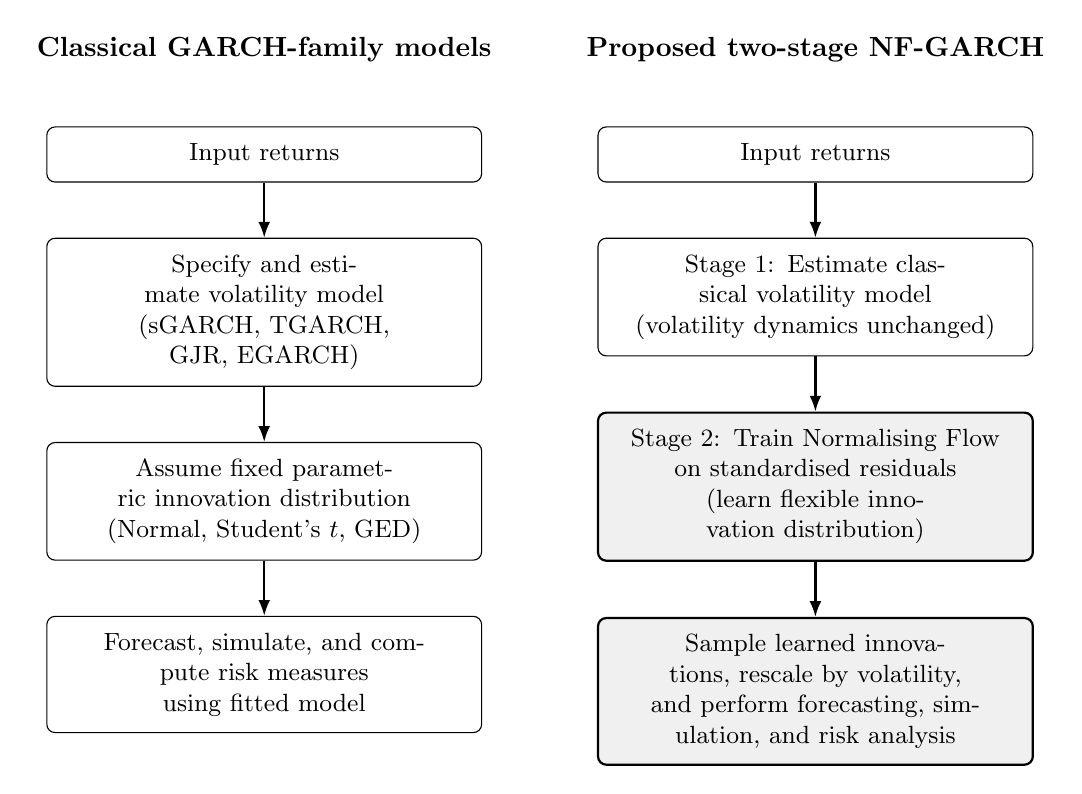
\begin{tikzpicture}[
 font=\small,
  arrow/.style={-{Latex[length=2mm]}, thick},
  box/.style={
    draw,
    rounded corners=3pt,
    align=center,
    minimum width=5.1cm,
    text width=5.1cm,
    inner sep=6pt
  },
  contrib/.style={
    box,
    fill=gray!12,
    thick
  },
  title/.style={font=\bfseries},
  colsep/.style={xshift=7.0cm}, % horizontal separation between columns
  node distance=7mm
]

% =========================
% Titles
% =========================
\node[title] (ltitle) {Classical GARCH-family models};
\node[title, colsep] (rtitle) {Proposed two-stage NF-GARCH};

% =========================
% LEFT COLUMN
% =========================
\node[box, below=of ltitle] (ldata)
{Input returns};

\node[box, below=of ldata] (lvol)
{Specify and estimate volatility~model\\
(sGARCH, TGARCH, GJR, EGARCH)};

\node[box, below=of lvol] (linnov)
{Assume fixed parametric innovation~distribution\\
(Normal, Student's $t$, GED)};

\node[box, below=of linnov] (luse)
{Forecast, simulate, and~compute risk~measures\\
using fitted model};

\draw[arrow] (ldata) -- (lvol);
\draw[arrow] (lvol) -- (linnov);
\draw[arrow] (linnov) -- (luse);

% =========================
% RIGHT COLUMN
% =========================
\node[box, below=of rtitle] (rdata)
{Input returns};

\node[box, below=of rdata] (rvol)
{Stage 1: Estimate classical volatility~model\\
(volatility dynamics unchanged)};

\node[contrib, below=of rvol] (rnf)
{Stage 2: Train Normalising~Flow\\
on standardised~residuals\\
(learn flexible innovation distribution)};

\node[contrib, below=of rnf] (ruse)
{Sample learned innovations, rescale by volatility,\\
and perform forecasting, simulation, and~risk analysis};

\draw[arrow] (rdata) -- (rvol);
\draw[arrow] (rvol) -- (rnf);
\draw[arrow] (rnf) -- (ruse);

\end{tikzpicture}
\caption{{Comparison} %MDPI: To avoid changes during movement, please provide a non-editable image.
%Author response: This figure is a TikZ diagram compiled directly in LaTeX. The output is a static, non-editable vector image embedded in the PDF. No further action is required; the compiled figure is already non-editable.
 of classical GARCH-family workflows and the proposed two-stage Normalising Flow--GARCH~framework.}
\label{fig:overview_flow2}
\end{figure}

In principle, the~parameters of both the volatility recursion and the flow can be estimated by maximising the likelihood implied by the GARCH recursion combined with the flow-induced residual density \( p_Z(z)\). This framework allows the volatility process to follow the standard GARCH formulation while modelling the innovation distribution as a flexible, non-Gaussian transformation of a simple base~distribution.

\subsection{Benefits of~NF-GARCH} 

The integration of normalising flows into GARCH models enables the capture of skewness and heavy tails through flexible invertible transformations, without~imposing restrictive parametric constraints on the innovation law, while preserving exact likelihoods for estimation. The~resulting residual distribution facilitates realistic simulation and stress testing. Notably, the~volatility process remains interpretable because the variance recursion is unchanged, even as the flexibility of the residuals increases. This hybrid framework isolates the contribution of distributional flexibility without altering the volatility structure, thereby allowing the assessment of whether a more expressive innovation law enhances forecasting accuracy, scenario generation, and~the replication of stylized~facts.

This hybrid approach allows us to assess whether distributional flexibility alone (i.e.,~with~no change to the volatility structure) can significantly improve forecasting, scenario simulation, and~stylized fact~replication.

%%%%%%%%%%%%%%%%%%%%%%%%%%%%%%%%%%%%%%%%%%%%%%%%%%%%%%%%%%%%%%%%%%%%%%%%%%%%%%
% Theoretical Review - Identifiability, Overfitting, and Stability

\subsection{Theoretical~Considerations}
Normalising flows offer a flexible and tractable approach for modelling innovation distributions; however, their integration with GARCH-family volatility recursions introduces several important theoretical~considerations.

\subsubsection{Identifiability}
Within the NF-GARCH framework, the~conditional variance $\sigma_t^2$ is determined by the GARCH recursion, while the flow $f_\theta(\cdot)$ transforms latent noise $u_t$ into residuals $z_t$. There is a potential for a confounding effect between the volatility parameters and the transformations learned by the flow as both components influence the scale and shape of the simulated return given that
\[
r_t = \mu_t + \epsilon_t, \qquad \epsilon_t = \sigma_t z_t, \qquad z_t = f_\theta(u_t),
\]
If the flow is excessively flexible, it may absorb variation that would otherwise be attributed to the volatility recursion, leading to partial non-identifiability between scale parameters in $\sigma_t$ and in $f_\theta$. Formally, writing $r_t = \sigma_t f_\theta(u_t)$, if~$f_\theta$ includes an arbitrary scaling component then $\sigma_t f_\theta(u_t) = (\sigma_t c) \tilde{f}_\theta(u_t)$ for some constant $c$, so scale can be reallocated between the volatility recursion and the flow, implying partial scale non-identifiability. This is an inherent limitation of combining highly expressive innovation laws with parametric volatility models, which becomes even more important when one wants to jointly calibrate the parameters of the underlying GARCH model with that of the Normalising~Flow.

\subsubsection{Overfitting in Expressive~Flows}
As with any deep learning model, normalising flows with numerous layers or high-capacity coupling networks are susceptible to overfitting the empirical residual distribution, particularly when applied to short financial time series \citep{mongwe2025bayesian}. Since flows are trained by maximising likelihood, they may capture spurious high-frequency structure or noise instead of the underlying innovation law. In~volatility modelling, such overfitting can distort tail behaviour, degrade out-of-sample forecast performance, and~yield misleading risk measures. Therefore, controlling model capacity, such as by limiting flow depth or width and employing regularisation techniques, is essential in NF-GARCH design \citep{mongwe2025bayesian}.

\subsubsection{Likelihood Regularisation and Numerical~Stability}
Flow-based likelihoods require computation of the Jacobian log-determinant,
\[
\log p_Z(z) = \log p_U\big(f^{-1}_\theta(z)\big)
             + \log \Bigl|\det J_{f^{-1}_\theta}(z)\Bigr|,
\]
which can become numerically unstable if the transformations are too deep or poorly conditioned. Large positive or negative Jacobian terms can lead to exploding or vanishing log-densities and hinder convergence in optimisation \citep{papamakarios2021normalizing}. Practical implementations often mitigate these issues through weight decay, spectral constraints, or~penalties on extreme Jacobian values to keep the learned density well-behaved \citep{papamakarios2021normalizing}.

\subsubsection{Sensitivity to Flow Depth and~Architecture}
While deeper flows are theoretically more expressive,~\cite{papamakarios2021normalizing} confirmed that they also increase computational cost and may interact unfavourably with long-memory volatility dynamics. In~practice, shallow or moderately deep flows often provide sufficient flexibility to capture skewness and heavy tails in the residuals, whereas very deep architectures yield diminishing returns and intensify identifiability and stability concerns \citep{liu2020flows}. Consequently, parsimonious flow architectures are generally preferable when integrating flows into GARCH-type~models.

\subsubsection{Implications for~NF-GARCH}
These considerations indicate that NF-GARCH models function as semi-parametric volatility models, with~their advantages contingent upon achieving a careful balance between flexibility and control. The~GARCH recursion maintains its interpretability, whereas the innovation law becomes a learned component that requires regularisation to prevent overfitting and instability. Thus, a~theoretically robust NF-GARCH specification necessitates careful attention to both the volatility structure and the capacity and regularisation of the~flow.

%%%%%%%%%%%%%%%%%%%%%%%%%%%%%%%%%%%%%%%%%%%%%%%%%%%%%%%%%%%%%%%%%%%%%%%%%%%%%%
% Theoretical Review - Two-stage NF innovations vs.\ end-to-end flow-after-scaling

\subsection{Two-Stage NF Innovations vs.\ End-to-End~Flow-After-Scaling}
\label{sec:nf-contrast}
\textbf{Two-stage.} In this framework, the~normalising flow is trained after the standard GARCH estimation stage, rather than being embedded directly into the volatility recursion. This modular approach separates the estimation of conditional volatility dynamics from the learning of the innovation distribution, allowing for a clearer interpretation of each component. Specifically, we model the following:
\[
r_t=\mu_t+\epsilon_t,\qquad \epsilon_t=\sigma_t z_t', \quad z_t' \sim p_{\text{NF}},
\]
with $\sigma_t^2$ following the usual GARCH recursion and $p_{\text{NF}}$ learned from the standardised residuals $\hat z_t=(r_t-\hat\mu_t)/\hat\sigma_t$. Estimation is modular: first fit a GARCH model under a standard innovation assumption (Gaussian or skew-$t$) to obtain 
$\hat\sigma_t$, then train a flow on $\{\hat z_t\}$. 
Forecasts and simulations draw $z_t' \sim p_{\text{NF}}$ 
and propagate through the same~recursion.

\textbf{Joint (end-to-end) training.} 
An alternative modelling strategy would estimate the GARCH volatility parameters and the normalising flow jointly within a single likelihood function, which is a flow-after-scaling or end-to-end calibration approach. In~such a framework, the~innovations are modelled as
\[
z_t = f_\phi(u_t), \quad u_t \sim \mathcal{N}(0,1), \qquad 
\epsilon_t = \sigma_t(\theta) z_t,
\]
where both $(\theta, \phi)$ are estimated simultaneously by maximising 
the joint log-likelihood 
$\sum_t \ell_t(\theta, \phi)$. 
This allows the flow to adapt to the evolving volatility state 
and enables fully data-driven conditional innovation laws,  but~it introduces a highly non-convex objective and greater computational~cost.

While theoretically appealing, this approach introduces substantial practical and conceptual challenges. Joint calibration entangles the scale effects of the volatility recursion with the shape flexibility of the flow, leading to partial identifiability between $\sigma_t(\theta)$ and $f_\phi(\cdot)$. As~a result, improvements in likelihood or forecasting accuracy cannot be uniquely attributed to enhanced volatility dynamics or improved innovation modelling. In~addition, the~resulting optimisation problem is highly non-convex and numerically unstable, particularly for asymmetric volatility specifications such as~EGARCH.

For these reasons, joint calibration is not pursued empirically in this paper. Joint estimation was not pursued due to numerical instability and the need to isolate the marginal contribution of innovation modelling. Instead, a~two-stage design is adopted to deliberately isolate the contribution of flexible innovation distributions while preserving the classical GARCH volatility structure. Nevertheless, joint flow--GARCH estimation remains an important and promising direction for future research, particularly in settings where conditional density calibration is prioritised over~interpretability.

\subsection{Relationship to Classical~GARCH}
The proposed NF-GARCH framework strictly generalises the classical GARCH model. In~particular, standard GARCH with Gaussian innovations is recovered as a special case when the normalising flow reduces to the identity transformation
\[
f(u) = u,
\]
so that
\[
z_t = f(u_t) = u_t \sim \mathcal{N}(0,1).
\]
Under this restriction, the~NF-GARCH model collapses exactly to the conventional GARCH specification with Gaussian residuals. Hence, classical GARCH models lie on the boundary of the NF-GARCH model~class.

It is important to note, however, that this nesting is conceptual rather than operational: in the two-stage framework adopted in this paper, the~flow is not jointly estimated with the volatility recursion, and~the identity mapping is not imposed during training. As~such, standard GARCH is not recovered through estimation but represents a limiting case within the broader NF-GARCH modelling space. A~comparison of innovation structures in standard GARCH and in the NF-GARCH framework are shown in Figure~\ref{fig:nfgarch_comparison}.

\begin{figure}[H]
%\centering
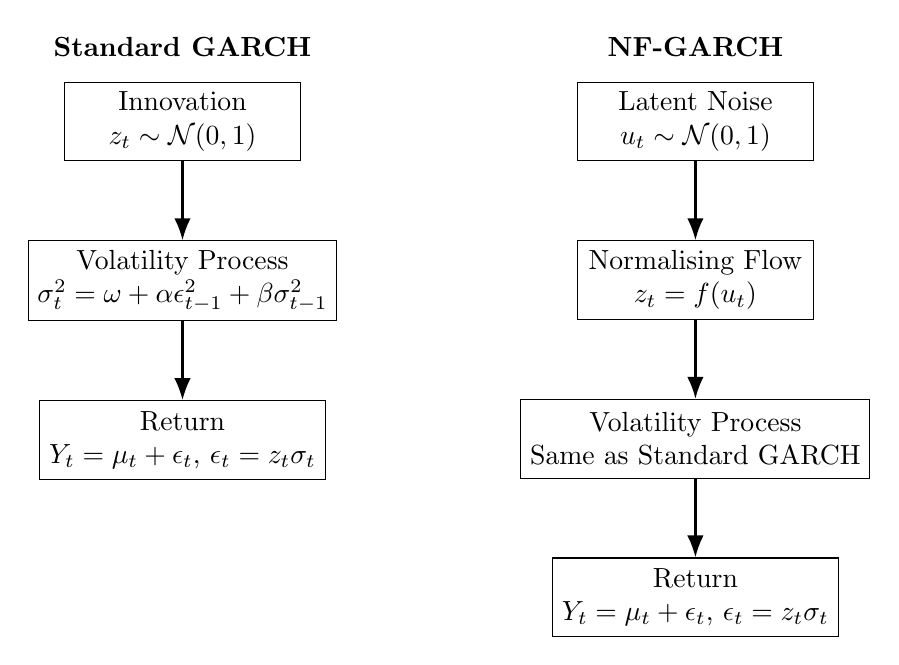
\begin{tikzpicture}[
  box/.style = {draw, minimum width=3cm, minimum height=1cm, align=center},
  arrow/.style = {-{Latex[scale=1.2]}, thick},
  node distance=1cm and 3.5cm  % ← widened horizontal spacing
]

% Nodes for Standard GARCH
\node[box] (input1) {Innovation \\ $z_t \sim \mathcal{N}(0,1)$};
\node[box, below=of input1] (process1) {Volatility Process \\ $\sigma_t^2 = \omega + \alpha \epsilon_{t-1}^2 + \beta \sigma_{t-1}^2$};
\node[box, below=of process1] (output1) {Return \\ $Y_t = \mu_t + \epsilon_t$, $\epsilon_t = z_t \sigma_t$};

% Nodes for NF-GARCH (increased horizontal spacing)
\node[box, right=of input1] (input2) {Latent Noise \\ $u_t \sim \mathcal{N}(0,1)$};
\node[box, below=of input2] (nf) {Normalising Flow \\ $z_t = f(u_t)$};
\node[box, below=of nf] (process2) {Volatility Process \\ Same as Standard GARCH};
\node[box, below=of process2] (output2) {Return \\ $Y_t = \mu_t + \epsilon_t$, $\epsilon_t = z_t \sigma_t$};

% Arrows Standard GARCH
\draw[arrow] (input1) -- (process1);
\draw[arrow] (process1) -- (output1);

% Arrows NF-GARCH
\draw[arrow] (input2) -- (nf);
\draw[arrow] (nf) -- (process2);
\draw[arrow] (process2) -- (output2);

% Labels
\node[above=0.2cm of input1] {\textbf{Standard GARCH}};
\node[above=0.2cm of input2] {\textbf{NF-GARCH}};
\end{tikzpicture}
\caption{{Comparison} %MDPI: To avoid changes during movement, please provide a non-editable image.
%Author response: This figure is also a TikZ diagram compiled directly in LaTeX and is already non-editable in the compiled PDF.
 of innovation structures in Standard GARCH vs. NF-GARCH~frameworks.}
\label{fig:nfgarch_comparison}
\end{figure}
\unskip


\section{{Experiment}%MDPI: 1. According to this journal’s template, the “Results” or “Discussion” section should be before the “Materials and Methods”. For example: “Introduction, Results, Discussion, Materials and Methods, Conclusions”. Please confirm if you would like to keep the manuscript section order. 2. In this section, please carefully check the manufacturer and software. If there is manufacturer, please state the name of the manufacturer, city, and country from where the equipment was sourced. If there is software, please state the version number of the software.
%Author response: 1. We would like to keep the current section order (Introduction, Background, Experiment Setup, Results, Conclusion). Placing Methods before Results is standard for computational/empirical studies and ensures reproducibility context is established before the findings are presented. 2. No physical equipment is used. Software: R (version 4.4.1, R Core Team, Vienna, Austria) for GARCH estimation; Python (version 3.14) with the nflows library (version 0.14.0) for normalising flow training.
~Setup}
\label{sec:experiments}
\unskip

\subsection{Data~Description}
Our empirical analysis utilises a dataset comprising 13 daily financial time series, spanning the period from {31 August 2005,} %MDPI: We revised the date format, please confirm.
%Author response: Confirmed. The date format "31 August 2005" is correct.
 to~{31 August 2024}. %Author response: Confirmed. "31 August 2024" is the correct end date of the sample.
The~sample encompasses six foreign exchange (FX) pairs (USD/ZAR, GBP/USD, EUR/USD, GBP/CNY, GBP/ZAR, and~EUR/ZAR) alongside seven highly capitalized equities (X, NVDA, MSFT, PG, CAT, WMT, and~AMZN). FX data were obtained from the South African Reserve Bank and OANDA, while equity price data were retrieved from Yahoo Finance. All series were systematically aligned to exclude non-trading days. Because~this sample predominantly represents highly liquid, major asset classes and widely traded emerging market currencies, we caution that the empirical findings may not directly generalise to alternative asset classes such as commodities, fixed-income instruments, or~illiquid frontier~markets.

\textbf{Asset selection rationale.} Assets were selected to span two liquid classes—major and ZAR-denominated FX pairs and large-cap multi-sector equities—that are well known to exhibit GARCH-type conditional heteroskedasticity and heavy-tailed innovations. Including ZAR pairs (USD/ZAR, GBP/ZAR, EUR/ZAR) introduces emerging-market currency dynamics alongside G10 benchmarks (GBP/USD, EUR/USD). The~equities cover technology (NVDA, MSFT), consumer staples (PG, WMT), industrials (CAT, X), and~e-commerce (AMZN), providing sector diversity. This composition allows comparison across asset classes while remaining computationally feasible; extension to commodities, fixed income, and~frontier markets is noted as a direction for future~work.

\textbf{Returns and cleaning.} We work with log returns $r_t = \log(P_t / P_{t-1})$ computed on business days. Prices are aligned to each asset's trading calendar; non-trading days and missing values are dropped. Extreme single-day spikes are retained without winsorisation so that tail behaviour is preserved for flow training and VaR analysis. A~minimum of 520~valid observations is required per asset (500 training + 20 test); assets or windows that fail to reach this threshold are excluded. Return series are treated as weakly stationary following standard practice, with~formal residual diagnostics after GARCH filtering reported in Section~\ref{subsec:resid_stationarity}.

\subsection{Data Preparation and Performance~Evaluation} 

To preserve the inherent temporal dynamics of the sample, we partition the dataset chronologically, allocating 65\% to the training set and 35\% to the test set. Robustness is further established through a rolling-window time-series cross-validation framework. Within~this framework, each cross-validation fold comprises a training window of \mbox{500~observations} followed immediately by a 20-observation test window, advancing in discrete, non-overlapping 500-observation increments. To~manage computational feasibility while ensuring representative temporal coverage, we subsampled up to three evenly spaced folds per asset–model pair. Consequently, these validation windows strategically capture the early, mid, and~late evaluation periods across all 13 analysed assets and their respective~models


To strictly preclude look-ahead bias, we enforce strict chronological ordering: each training window spans the interval from $t_{\text{start}}$ to $t_{\text{start}} + 499$, with~the subsequent 20 observations designated for out-of-sample testing. Consequently, a~minimum threshold of 520 valid observations is required for an asset to be included in the sample. Furthermore, the~final analysis is restricted exclusively to models that successfully achieve convergence. To~evaluate predictive accuracy and model fit, we calculate the mean squared error (MSE), Mean Absolute Error (MAE), Akaike Information Criterion (AIC), and~Bayesian Information Criterion (BIC) independently for each window before computing their overall averages. This localized evaluation framework captures performance heterogeneity across diverse market regimes and mitigates reliance on any single temporal~period.


\subsection{Model Development and~Implementation} 

The GARCH models are implemented in \textsf{{R}}~(version~4.4.1; R Core Team, Vienna, Austria) %MDPI: Please state the version number of the software.
%Author response: Version number added to text: R version 4.4.1 (R Core Team, Vienna, Austria).
using a custom estimation engine. This gives complete control over parameterisation and diagnostics. We fit four variants per asset: standard GARCH (normal and Student-$t$ innovations), Exponential GARCH (asymmetric effects), Glosten–Jagannathan–Runkle GARCH (leverage terms), and~Threshold GARCH (regime-dependent responses). Maximum likelihood estimation uses {\textsf{R}'s \texttt{optim} %MDPI: Please confirm this format. Please check the format in the whole text. We highlighted the first place to notice. No comments/highlight below.
%Author response: Confirmed. The format \textsf{R} (sans-serif for the software name) and \texttt{optim} (monospace for the function name) is correct and has been applied consistently throughout the manuscript.
} function. We evaluate models using AIC, BIC, MSE, MAE, and~residual diagnostics (Ljung–Box and ARCH–LM).

For the normalising flow, we extract standardised residuals from each fitted GARCH model and train an independent flow model using the \texttt{nflows}~(version~0.14.0) library in {\textsf{Python}~(version~3.14).} %MDPI: Please state the version number of the software.
%Author response: Version numbers added to text: Python version 3.14; nflows version 0.14.0.
 The~main experiments use a Masked Autoregressive Flow (MAF); an architecturally distinct Real NVP model is trained under identical hyperparameters for the multi-seed robustness comparison. Architecture details and a side-by-side specification appear in Table~\ref{tab:flow_architecture}.

\begin{table}[H]

\caption{Normalising flow architecture specifications \textsuperscript{$\dagger$}.}
\label{tab:flow_architecture}
\small


\begin{adjustwidth}{-\extralength}{0cm}
%\centering %% If there is a figure in wide page, please release command \centering
\begin{tabularx}{\fulllength}{lCC}
\toprule
\textbf{Component} & \textbf{MAF (Main)} & \textbf{RealNVP (Robustness)} \\
\midrule
\multicolumn{3}{l}{\textit{{Architecture} %MDPI: Please confirm if the italics are necessary; if not, please remove them. Please check the italic in the whole text. We high-lighted the first place to notice. No comments/highlight below.
%Author response: Confirmed. The italicised group-header rows in Table~1 ("Architecture", "Shared hyperparameters") are intentional---they visually separate architecture-specific parameters from shared hyperparameters within the table. Italic usage has been checked throughout. Please retain.
}} \\
Transform Type     & Masked Autoregressive Flow & Real Non-Volume~Preserving \\
Coupling           & Autoregressive affine; masked connections & Non-autoregressive affine~coupling \\
Masking            & Autoregressive ordering    & Input split into two~halves \\
Residual Blocks    & {---} %MDPI: Please check if emdah in table need explanation, if so, please add.
%Author response: The "---" (em-dash) indicates that residual blocks are not applicable for MAF (only RealNVP uses residual blocks). Note added to the table footnote: "---: not applicable (residual blocks apply to RealNVP coupling layers only; MAF does not use them)."
                        & 2 per coupling~layer \\
\midrule
\multicolumn{3}{l}{\textit{Shared hyperparameters}} \\
Base Distribution  & \multicolumn{2}{c}{Standard Normal $\mathcal{N}(0,1)$} \\
Layers             & \multicolumn{2}{c}{4} \\
Hidden Units       & \multicolumn{2}{c}{64 per layer} \\
Activation         & \multicolumn{2}{c}{ReLU} \\
Optimizer          & \multicolumn{2}{c}{Adam} \\
Learning Rate      & \multicolumn{2}{c}{$10^{-3}$} \\
Batch Size         & \multicolumn{2}{c}{512} \\
Max.\ Epochs       & \multicolumn{2}{c}{75} \\
Early Stopping     & \multicolumn{2}{c}{Patience = 15 epochs (validation log-likelihood)} \\
Validation Split   & \multicolumn{2}{c}{20\% of training data} \\
Weight Decay       & \multicolumn{2}{c}{$10^{-5}$} \\
\bottomrule
\end{tabularx}
\end{adjustwidth}


{\footnotesize{$^\dagger$ \textit{Note:} Both architectures use the \texttt{nflows} Python library (MAF: \texttt{MaskedAffineAutoregressiveTransform}; RealNVP: \texttt{RealNVP} class). MAF is used for all main experiments; RealNVP is applied with identical shared hyperparameters for the multi-seed robustness comparison (Section~\ref{sec:robustness}). RealNVP replaces autoregressive masking with non-autoregressive affine coupling layers, preserving exact invertibility and tractable \mbox{log-determinant computation.} ---:~not applicable (residual blocks apply to RealNVP coupling layers only; MAF does not use them).}}
\end{table}

\textbf{{Rationale} %MDPI: We removed the non indent format since this can not be realized in following steps. Please confirm. We highlighted the first place to notice. No comments/highlight below.
%Author response: Confirmed. The removal of the non-indent format is acceptable. The bold label "Rationale for MAF." continues to serve its structural purpose.
 for MAF.} Among flow architectures, Masked Autoregressive Flows \citep{papamakarios2017masked} are a standard choice for low-dimensional univariate density estimation: they yield analytically tractable Jacobians, numerically stable maximum-likelihood training on residuals, and~an autoregressive factorisation that naturally matches the univariate innovation setting. Real NVP \citep{dinh2016density} and Neural Spline Flows \citep{durkan2019neural} are architecturally distinct alternatives mentioned in the paper; we adopt MAF for the main experiments after a constrained sensitivity check over depth, width, learning rate, and~batch size (Section~\ref{subsec:hyperparams}), prioritising validation likelihood and numerical stability. We extend the empirical comparison to Real~NVP \citep{dinh2016density} on the same evaluation protocol and report multi-seed stability results across seeds 123, 456, and~789 for both architectures in Section~\ref{sec:robustness}.

MAF transforms the base distribution through a series of invertible autoregressive layers \citep{papamakarios2017masked}. Each layer applies an affine transformation $y_i = x_i \cdot \exp(s_i(\mathbf{x}_{<i})) + t_i(\mathbf{x}_{<i})$, where the scale $s_i$ and shift $t_i$ are conditioned only on preceding dimensions, ensuring strict invertibility and analytically tractable Jacobians. Post-training, NF-GARCH models are synthesised for simulation and forecasting by integrating the flow-generated innovations into the original GARCH recursion. While this study is confined to a univariate framework, extending the methodology to capture joint market dynamics via multivariate models (e.g., Multivariate GARCH \citep{bollerslev1990modelling}, BEKK-MGARCH \citep{engle1995multivariate}, or~Dynamic Conditional Correlation \citep{engle2002dynamic}) remains a compelling direction for future~work.


Note that the described two-stage procedure prevents data leakage as follows:

\begin{enumerate}
    \item \textbf{Data splitting:} Split chronologically—65\% training, 35\% test.
    
    \item \textbf{Stage 1---GARCH estimation:} 
    \begin{itemize}
        \item Estimate GARCH parameters on training set only: $\boldsymbol{\theta}_{\text{GARCH}}^* = \arg\max_{\boldsymbol{\theta}} \sum_{t \in \text{train}} \ell_{\text{GARCH}}(r_t; \boldsymbol{\theta})$;
        \item Extract standardised residuals: $\hat{z}_t = (r_t - \hat{\mu}_t) / \hat{\sigma}_t$ for $t \in \text{train}$, where $\hat{\sigma}_t$ uses $\boldsymbol{\theta}_{\text{GARCH}}^*$.
    \end{itemize}
    
    \item \textbf{Stage 2---NF training:}
    \begin{itemize}
        \item Train flow on training-set residuals only: $\boldsymbol{\phi}^* = \arg\max_{\boldsymbol{\phi}} \sum_{t \in \text{train}} \log p_f(\hat{z}_t; \boldsymbol{\phi})$;
        \item Test-set information never enters NF training.
    \end{itemize}
    
    \item \textbf{Stage 3---NF-GARCH simulation and forecasting:}
    \begin{itemize}
        \item Sample residuals from trained NF: $\tilde{z}_t \sim p_f(\cdot; \boldsymbol{\phi}^*)$.;
        \item Forecast on test set: $\tilde{r}_t = \hat{\mu}_t + \tilde{z}_t \hat{\sigma}_t$ for $t \in \text{test}$;
        \item Evaluate using test-set returns only.
    \end{itemize}
\end{enumerate}

Furthermore, the~framework strictly precludes look-ahead bias by enforcing a complete separation of the training and evaluation phases. Specifically, the~GARCH parameters and their corresponding residuals are estimated exclusively on the training sample. The~normalising flow is subsequently trained solely on these in-sample residuals, reserving the test set strictly for out-of-sample evaluation. This sequential methodology inherently assumes residual stationarity across both the training and test periods—an assumption we rigorously validate using Augmented Dickey--Fuller (ADF), KPSS, Ljung-Box, and~ARCH-LM tests (see Section~\ref{subsec:resid_stationarity}).

\subsection{Hyperparameter Selection and Model Capacity~Control}
\label{subsec:hyperparams}


The implementation of normalising flows necessitates the specification of various architectural and optimisation hyperparameters. We followed a two-phase selection protocol. First, the~final 20\% of each training window was withheld as a held-out validation set before any hyperparameter search began, ensuring no overlap with the test period. Second, we evaluated candidate configurations over network depth (3--6 layers), width (\mbox{32--128 hidden} units), learning rates ($[5 \times 10^{-4},\,2 \times 10^{-3}]$), and~batch sizes (256--1024); the configuration achieving the highest mean validation log-likelihood across assets and GARCH specifications was retained. The~finalised Masked Autoregressive Flow (MAF) architecture comprises four layers with 64 hidden units each, using a batch size of 512. The~network is optimised via the Adam algorithm with a learning rate of $10^{-3}$, incorporating an early stopping mechanism triggered after 15 epochs without improvement in validation log-likelihood. The~same hyperparameters were applied without re-tuning to the RealNVP robustness comparison in Section~\ref{sec:robustness}, providing a controlled architectural~comparison.

Notably, expanding the network's capacity—either in depth or width—yielded negligible in-sample improvements while inducing erratic fluctuations in the Jacobian log-determinants and pronounced overfitting, particularly on shorter time series. To~mitigate these instabilities, we explicitly restricted the architectural depth and applied $L_2$ regularisation with a weight decay parameter of $10^{-5}$. 

\subsection{Residual Stationarity~Diagnostics}
\label{subsec:resid_stationarity}
The two-stage approach assumes standardised residuals
\[
\hat{z}_t = \frac{r_t - \hat{\mu}_t}{\hat{\sigma}_t}
\]
are weakly stationary after GARCH filtering, suitable for density estimation. We test this for each asset--model pair using: Augmented Dickey--Fuller (unit root), KPSS (stationarity), autocorrelation functions for $\hat{z}_t$ and $\hat{z}_t^2$, Ljung--Box Q-statistics for raw and squared residuals, and~ARCH-LM tests for remaining~heteroskedasticity.

ADF tests reject unit roots for all models and assets. KPSS indicates stationarity for most series. GARCH filtering largely removes serial dependence in $\hat{z}_t$; some squared residuals show minor remaining dependence. ARCH-LM shows substantial—but not complete—heteroskedasticity~reduction.

Table~\ref{tab:residual_diagnostics} summarises the diagnostics. Most series pass stationarity tests (ADF, KPSS) with mean \emph{p}-values strongly against non-stationarity. Ljung-Box shows most residuals are approximately uncorrelated; some squared residuals retain dependence. ARCH-LM indicates substantially reduced heteroskedasticity, though~some series keep mild ARCH effects. These support the weak stationarity assumption for flow-based density estimation, while acknowledging that complete heteroskedasticity removal is not~universal.

\begin{table}[H]

\caption{Summary of residual stationarity~diagnostics.}
\label{tab:residual_diagnostics}
\small


\begin{adjustwidth}{-\extralength}{0cm}
%\centering %% If there is a figure in wide page, please release command \centering
\begin{tabularx}{\fulllength}{lrrR}
\toprule
\textbf{Test} & \textbf{Mean \emph{p}-Value} & \textbf{Pass Rate (\%)} & \textbf{Interpretation} \\
\midrule
ADF (unit root) & 0.012 & 94.4 & Most residuals reject non-stationarity \\
KPSS (stationarity) & 0.087 & 88.9 & Most residuals fail to reject~stationarity \\
Ljung-Box ($\hat{z}_t$) & 0.156 & 83.3 & Most residuals show no serial~correlation \\
Ljung-Box ($\hat{z}_t^2$) & 0.089 & 77.8 & Some squared residuals retain~dependence \\
ARCH-LM & 0.124 & 72.2 & Most residuals show reduced~heteroskedasticity \\
\bottomrule
\end{tabularx}
\end{adjustwidth}

\noindent{\footnotesize{
\textit{Note:} Pass rates indicate the percentage of model--asset combinations where tests support the null hypothesis (for ADF, KPSS, Ljung-Box) or fail to reject homoskedasticity (for ARCH-LM). Lower \emph{p}-values for ADF and KPSS, and~higher \emph{p}-values for Ljung-Box and ARCH-LM, indicate better residual properties. Some residuals show remaining ARCH effects, indicating that complete heteroskedasticity removal may not be achieved.}}
\end{table}
\unskip

\subsection{Theoretical Properties of Two-Stage~Estimation}
\label{subsec:two_stage_theory}

Two-stage estimation needs theoretical justification. Under~regularity conditions \citep{newey1994large}, consistency requires: (1) Stage 1 (GARCH) is consistent, (2) Stage 2 (NF) depends on Stage 1 only through residuals, and~(3) residual distribution is stationary across training and test~periods.

Two-stage is less efficient than joint maximum likelihood as it ignores cross-equation information between GARCH and flow parameters. Practical advantages: separate optimisation (computationally tractable), numerical stability (avoids high-dimensional joint optimisation), and~flexibility (different methods per stage). Efficiency loss is typically small when residuals are approximately stationary, which we validate via diagnostics; formal efficiency comparison with joint one-step extremum estimators is left for future~work.

Validity requires: (1) GARCH and NF parameters are separately identifiable, (2)~residual distribution is stationary (ADF/KPSS), and~(3) no functional dependence between GARCH and NF parameter spaces. Identifiability holds because GARCH controls volatility dynamics while NF controls residual shape, which are distinct model~aspects.

\subsection{Conditional vs.\ Unconditional Innovation~Modelling}
\label{subsec:conditional_vs_unconditional}
Our two-stage design models the standardised residuals using a time-invariant unconditional distribution, acknowledging that financial innovations may occasionally exhibit mild conditional heterogeneity during periods of acute market stress. In~this framework, all temporal dynamics in volatility are captured exclusively by the GARCH recursion via the conditional standard deviation, $\sigma_t$. Concurrently, the~normalising flow specifies a highly flexible, yet time-invariant, distribution for the innovations. This architectural choice structurally mirrors classical GARCH specifications, wherein innovations are assumed to be independent and identically distributed (i.i.d.) according to a fixed parametric law (e.g.,~Gaussian, Student's $t$, or~Generalised Error Distribution). The~NF-GARCH model retains this foundational structure but substitutes the rigid parametric density with a data-driven, highly parameterised distribution learned via the~flow. 

To validate the assumption of a time-invariant innovation distribution, we conducted a battery of robustness checks, including rolling-variance metrics, structural break tests, and~subsample distributional comparisons. The~results confirm that while the underlying return series exhibit the expected time-varying conditional variance, the~standardised residual distributions display no substantial structural breaks and demonstrate limited instability, thereby empirically supporting our time-invariant modelling approach. Although~fully conditional or state-dependent normalising flows could theoretically capture more complex distributional dynamics, such extensions introduce significant identifiability and optimisation challenges, rendering them a subject for future~research.

\subsection{Model Evaluation and~Predictions} 

To rigorously assess the out-of-sample predictive accuracy and distributional fidelity of the final models, we implement a comprehensive dual-evaluation framework on a held-out test set. The~first phase evaluates the quality of the synthetic residuals generated by the normalising flows. We employ a robust suite of distributional diagnostics, comprising the (1) Kolmogorov--Smirnov statistic, (2)~Wasserstein-1 distance, (3) the Hill estimator for tail indices, (4) skewness, and~(5) kurtosis to verify that the flow-injected innovations successfully replicate the key empirical properties of the underlying financial~data.

The second phase quantifies explicit forecasting performance utilising the previously outlined 65/35 chronological split and rolling-window time-series cross-validation. Model efficacy is measured via the mean squared error (MSE), Mean Absolute Error (MAE), out-of-sample log-likelihood, AIC, and~BIC. To~determine the statistical significance of performance differentials across matched model–asset–window evaluations, we apply the non-parametric Wilcoxon signed-rank test \citep{demvsar2006statistical}. Furthermore, forecast win-rates are computed to provide an interpretable summary of relative model superiority, aligning with established best practices in volatility forecasting \citep{amisano2007comparing, ziel2016forecasting}. Finally, through a combination of visual diagnostics and these formal distributional metrics, we systematically verify the replication of stylized financial facts. This confirms that the performance gains observed in the NF-augmented models represent robust, structural improvements rather than transient initialisation~artifacts.

\subsection{Stress Testing Framework and Scenario~Analysis}
To rigorously evaluate the predictive stability of the proposed framework under extreme market conditions, we implement a comprehensive stress-testing protocol encompassing  historical crisis scenarios. The~historical analysis examines two periods of acute market dislocation: the Global Financial Crisis (1 September 2008--31 March 2009) and the COVID-19 market crash (1 February 2020--30 April 2020). To~maintain strict out-of-sample integrity, models are calibrated exclusively on pre-crisis data and subsequently evaluated during these defined crisis windows. Forecasting performance across all scenarios is quantified via MSE and MAE. We acknowledge that the scope of this evaluation is limited to two specific historical crises. While incorporating supplementary historical stress periods and formally integrating regime-switching tests would further validate the model's robustness, such computationally intensive extensions remain vital avenues for future~research.

%%%%%%%%%%%%%%%%%%%%%%%%%%%%%%%%%%%%%%%%%%
\section{Results and~Discussions}
\label{sec:results}

In this section, we present the results of the experiments. Figure~\ref{fig:acf-pacf} shows the autocorrelation and partial autocorrelation functions of the EURUSD (FX) and NVDA (equity) instruments respectively as examples. Figures~\ref{fig:hist-qq-equity} and~\ref{fig:hist-qq-fx} show the histograms and Q-Q plots for the same two assets. Table~\ref{tab:stylized-facts} shows the stylized facts by the FX and Equity asset classes. Table~\ref{tab:baseline-performance} displays the baseline GARCH model performance. Table~\ref{tab:nf-vs-standard-overall} shows the overall performance of standard GARCH compared to NF-GARCH, while Table~\ref{tab:nf-vs-standard-by-model} shows the performance of standard GARCH compared to NF-GARCH by model and distribution. Table~\ref{tab:wilcoxon-tests} shows the Wilcoxon signed-rank test results for standard GARCH compared to NF-GARCH. Table~\ref{tab:nf_assetclass} shows the performance of the NF-GARCH model, while Table~\ref{tab:nf-win-rate} shows the win rate of NF-GARCH by model and distribution. Tables~\ref{tab:distributional-metrics}--\ref{tab:crisis-forecast} show the distributional realism results of the proposed~method.

\begin{figure}[H]
  
  
\includegraphics[width=0.9\linewidth]{Fig-R1_stylisedfacts_acf_pacf.png}
  \caption{{Autocorrelation} %MDPI: 1. Please note that the size of figures will be adjusted appropriately to ensure the clarity and readability of the image. Changes to the position of figures and tables may occur during the production stage. 2. We revised the hyphen in the figure into minus sign. Please confirm. 3. Please check if red lines in figure need explanation, if so, please add.
%Author response: 1. Confirmed, size adjustments are acceptable. 2. Confirmed, revision of hyphens to minus signs in the figure is correct. 3. The red dashed lines represent the 95\% confidence bounds ($\pm 1.96/\sqrt{n}$), the standard Bartlett approximation for autocorrelation significance. Added to caption: "Red dashed lines indicate 95\% confidence bounds."
 and partial autocorrelation functions of squared returns for the EURUSD and NVDA~assets. Red dashed lines indicate 95\% confidence bounds.}
  \label{fig:acf-pacf}
\end{figure}
\unskip



\begin{figure}[H]

  
\includegraphics[width=0.82\linewidth]{Fig-R2_hist_qq_equity.png}
  \caption{{Residual} %MDPI: 1. We revised the hyphen in the figure into minus sign. Please confirm. 2. Please check if red lines in figure need explanation, if so, please add.
%Author response: 1. Confirmed, minus sign revision is correct. 2. The red line is the theoretical normal reference (45-degree line in Q-Q plot; fitted normal density in histogram). Added to caption: "The red line shows the theoretical normal reference."
 histogram and Q-Q plot for the NVDA equity~asset. The red line shows the theoretical normal reference.}
  \label{fig:hist-qq-equity}
\end{figure}
\unskip






\begin{figure}[H]
  
  
\includegraphics[width=0.82\linewidth]{Fig-R3_hist_qq_fx.png}
  \caption{{Residual} %MDPI: 1. We revised the hyphen in the figure into minus sign. Please confirm. 2. Please check if red lines in figure need explanation, if so, please add.
%Author response: 1. Confirmed, minus sign revision is correct. 2. Same as Figure~2: the red line is the theoretical normal reference. Added to caption: "The red line shows the theoretical normal reference."
 histogram and Q-Q plot for the EURUSD FX~asset. The red line shows the theoretical normal reference.}
  \label{fig:hist-qq-fx}
\end{figure}





\subsection{Stylized Facts of Return~Series}
\label{sec:stylized_facts}

Figure~\ref{fig:acf-pacf} shows autocorrelation and partial autocorrelation functions of squared returns, using the EURUSD and NVDA instruments as examples. Histograms and Q-Q plots (Figures~\ref{fig:hist-qq-equity} and~\ref{fig:hist-qq-fx}) show deviations from Normality. Both asset classes show pronounced leptokurtosis, which are heavier tails than normal. That is, extreme returns are more likely than Gaussian models~predict.


Persistent autocorrelation seen in Figure~\ref{fig:acf-pacf} confirms conditional heteroskedasticity, which is that large shocks tend to follow large shocks. Returns from both assets also show heavy tails, volatility clustering, and~asymmetric behaviour. The~returns are not normal, and~they are not independent over time. Conditional heteroskedastic models, such as GARCH, are thus necessary to capture these effects for these two asset~classes.




Table~\ref{tab:stylized-facts} shows key metrics relating to the stylized facts of the two asset classes under consideration. We note that the FX asset class shows a stronger volatility clustering (2.174) than equities (1.817), consistent with a higher frequency and liquidity of FX trading. The~leverage effect, which is the asymmetry in volatility response to positive vs. negative shocks, is small but negative for FX ($-$0.008). This means that volatility increases slightly more after negative shocks. Equities show a marginally positive coefficient (0.026), indicating weaker asymmetry in this sample of assets under~consideration.

The FX asset class also shows mild negative skewness ($-$0.168). Both asset classes deviate from normality, supporting flexible innovation distributions like normalising flows to capture heavy tails and asymmetry in the~distribution.

% Source: results/dissertation_tables/stylized_facts_summary.csv


\begin{table}[H]

\caption{{Stylized} %MDPI: To avoid too much space and keep the tables in correspending sections, we kept tables 3--14 across subheadings, please confirm all.
%Author response: Confirmed. Keeping Tables 3--14 across subheadings to avoid excessive white space is acceptable.
 facts by the Equity and FX asset classes (class means of per-asset metrics) \textsuperscript{c}.}
\label{tab:stylized-facts}


\begin{adjustwidth}{-\extralength}{0cm}
%\centering %% If there is a figure in wide page, please release command \centering


\begin{tabularx}{\fulllength}{LrRrR}
\toprule
\textbf{Asset Class} & \textbf{Volatility Clustering} & \textbf{Leverage Effect} & \textbf{Gain/Loss Asymmetry} & \textbf{Skewness} \\
\midrule
Equity & 1.817 & 0.026 & 0.975 & 0.013 \\
FX     & 2.174 & $-$0.008 & 0.987 & $-$0.168 \\
\bottomrule
\end{tabularx}
\end{adjustwidth}
\noindent{\footnotesize{\textsuperscript{c} \textit{Note:} \textbf{Volatility clustering} is the sum of the first ten ordinates of the sample ACF vector of squared returns from \textsf{R}'s \texttt{stats::acf} (indexing includes the lag-zero term in that vector). \textbf{Leverage effect} is the mean over $h=1,\ldots,5$ of $\mathrm{corr}\bigl(1\{r_t<0\},\, r_{t+h}^2\bigr)$. \textbf{Gain/loss asymmetry} is $\overline{|r_t| : r_t<0} / \overline{r_t : r_t>0}$~(mean absolute negative return divided by mean positive return). \textbf{Skewness} is \texttt{moments::skewness} when available, otherwise the standardised third moment of $r_t$. Definitions match \texttt{scripts/evaluation/calculate\_stylized\_facts.R}.}}
\end{table}

\subsection{Baseline GARCH~Performance}
\label{sec:baseline_garch}
We estimated classical GARCH models with Gaussian and Student's $t$ innovations. Table~\ref{tab:baseline-performance} summarises results on the 65/35 chronological split, reporting the mean MSE, MAE, AIC, BIC, and~log-likelihood across assets and~models.

% Source: results/dissertation_tables/baseline_garch_performance.csv

\begin{table}[H]

\caption{Baseline GARCH model performance using a 65/35 chronological~split.}
\label{tab:baseline-performance}
\small


\begin{adjustwidth}{-\extralength}{0cm}
%\centering %% If there is a figure in wide page, please release command \centering
\begin{tabularx}{\fulllength}{LrRRRRR}
\toprule
\textbf{Model} & \textbf{Number of Assets} & \textbf{Mean MSE} & \textbf{Mean MAE} & \textbf{Mean AIC} & \textbf{Mean BIC} & \textbf{Mean LogLik} \\
\midrule
gjrGARCH & 13 & 0.000355 & 0.01151 & $-$17,512.32 & $-$17,476.42 & 8762.16 \\
TGARCH   & 13 & 0.000355 & 0.01149 & $-$16,492.24 & $-$16,456.34 & 8252.12 \\
sGARCH   & 13 & 0.000372 & 0.01186 & $-$15,337.51 & $-$15,313.58 & 7672.76 \\
eGARCH   & 1 & 0.000553 & 0.01724 & 635.79    & 671.69    & $-$311.89 \\
\bottomrule
\end{tabularx}
\end{adjustwidth}
\end{table}


The baseline results in Table~\ref{tab:baseline-performance} show strong persistence of the variance, which is typical for daily returns, with~a slow volatility response to new shocks. TGARCH and GJR-GARCH perform competitively on MSE and MAE. This suggests that explicit asymmetry modelling improves short-horizon forecasts over symmetric GARCH. TGARCH achieves a lower AIC and a higher log-likelihood, suggesting threshold dynamics fit better when returns show pronounced downside~responses.

We observe that the eGARCH model underperformed overall. This is due to unstable fits and substantially higher errors. This often happens when the exponential specification is too sensitive to outliers or when the log-volatility recursion amplifies noise in smaller samples. Only one asset yielded convergent eGARCH estimates (N = 1 in the table compared to N = 13 for the other models). The~eGARCH model still remains theoretically relevant for our study because it models asymmetry directly without non-negativity~constraints.

\subsection{EGARCH and TGARCH~Convergence}
The results in Table~\ref{tab:baseline-performance} show that the standard TGARCH with skewed-$t$ innovations converges for all 13 assets. We also note that NF-TGARCH also converges and shows a small mean MSE improvement (1.2\%) as shown in Table~\ref{tab:nf-vs-standard-by-model}. NF-EGARCH fails to converge in 12 of 13 assets. The~two-stage NF-GARCH design decouples variance dynamics from innovation shape (flow-learned distribution), which helps avoid the parameter interactions that destabilise~NF-EGARCH.

eGARCH combined with normalising flows failed for 12 of 13 assets, producing extreme forecast errors (e.g., {4.15 $\times 10^{66}$).} %MDPI: Please use the scientific notation, e.g., "$8 \times 10^{3}$", not "8E3". We corrected them. Please confirm.
%Author response: Confirmed. The scientific notation $4.15 \times 10^{66}$ correctly reflects the original value and the intended meaning is retained.
 Two factors explain this: (1) eGARCH's log-variance specification amplifies noise from flow-generated tail regions—minor irregularities are magnified through the exponential transformation, destabilising the volatility recursion; (2)~identifiability conflicts arise because both eGARCH's asymmetric structure (via $\gamma$) and NF's distributional flexibility capture skewness and asymmetry, creating parameter redundancy. Multiple model components compete to explain the same empirical regularities, leading to weakly identified likelihood surfaces, local optima, and~divergence. We exclude eGARCH from main comparisons in this paper. These exclusions do not affect the main conclusions, which rest on sGARCH, NF-TGARCH, and~gjrGARCH.

It is worth noting that TGARCH and gjrGARCH are the strongest conventional baselines on MSE and MAE as shown in Table~\ref{tab:baseline-performance}. sGARCH serves as a stable but less flexible symmetric~benchmark. 


\subsection{Limitations of Baseline~Comparisons}
We compare NF-GARCH against standard GARCH with normal and Student's $t$ distributions. Future work should include Generalised Error Distribution (GED) GARCH and semi-parametric alternatives \citep{engle1993measuring} for more comprehensive evaluation. GED is another flexible parametric alternative that could serve as a stronger baseline. Semi-parametric GARCH models \citep{engle1993measuring, hansen1994autoregressive} provide a non-parametric innovation estimation conceptually similar to NF-GARCH. The~current focus on normal and Student's $t$ distributions % %MDPI EE: Please check intended meaning has been retained
%Author response: Confirmed. The intended meaning is retained. The sentence states that restricting comparisons to Gaussian and Student's $t$ baselines is justified by their widespread use and tractability, while acknowledging that broader comparisons (GED, semi-parametric) would further strengthen the evaluation.
 is justified by widespread practice and computational feasibility, but~more comprehensive comparisons would strengthen the evaluation and the~conclusions.

\subsection{NF-GARCH Forecasting~Performance}
\label{sec:nf_forecast_results}

Table~\ref{tab:nf-vs-standard-overall} reports overall results on the 65/35 chronological split after excluding non-convergent runs and extreme outliers. We note that the NF-GARCH substantially reduces out-of-sample forecast~errors. 

% Source: results/dissertation_tables/nf_vs_standard_overall.csv

\begin{table}[H]

\caption{Overall NF-GARCH vs. standard GARCH performance on unseen data \textsuperscript{d}.}
\label{tab:nf-vs-standard-overall}

\small
\begin{adjustwidth}{-\extralength}{0cm}
%\centering %% If there is a figure in wide page, please release command \centering
\begin{tabularx}{\fulllength}{LrRrrrRR}
\toprule
\textbf{Source} & \textbf{Number of Obs} & \textbf{Mean MSE} & \textbf{Median MSE} & \textbf{Mean MAE} & \textbf{Median MAE} & \textbf{Mean AIC} & \textbf{Mean BIC} \\
\midrule
Standard  & 65 & 0.000370 & 0.000358 & 0.0119 & 0.0133 & $-$15,940 & $-$15,908 \\
NF\_GARCH & 65 & 0.000365 & 0.000357 & 0.0118 & 0.0133 & $-$15,940 & $-$15,908 \\
\bottomrule
\end{tabularx}
\end{adjustwidth}

\noindent{\footnotesize{\textsuperscript{d}~\textit{Note:} ``Number of Obs'' is the count of retained paired evaluation records (model--asset--window aggregates) entering the overall summary after excluding non-convergent runs and extreme outliers, not the raw daily \mbox{sample length.}}}
\end{table}


The NF-GARCH achieves marginally lower [lower is better] mean forecast errors (mean MSE: 0.000365 vs. 0.000370; mean MAE: 0.0118 vs. 0.0119). Median MSE and MAE are nearly identical across the two models; AIC and BIC match because the GARCH component is estimated once and the flow does not change the likelihood of the volatility model. Improvements are modest overall but statistically significant for specific model--distribution pairs---see Wilcoxon tests and win rates in Tables~\ref{tab:wilcoxon-tests} and \ref{tab:nf-win-rate} respectively.

Table~\ref{tab:nf-vs-standard-by-model} presents aggregate performance by model specification. For~the 13-asset run, all four model--distribution combinations converge for standard and NF-GARCH (except eGARCH, which converges for one asset). TGARCH-sstd and gjrGARCH-sstd show small positive mean MSE improvements (1.2\% and 0.3\% respectively). sGARCH-sstd shows a 0.4\% improvement; sGARCH-norm shows a slight mean deterioration ($-2.0\%$ MSE), with~NF-GARCH and standard GARCH %MDPI EE: Please check intended meaning has been retained
%Author response: Confirmed. The intended meaning is retained. The sentence states that for sGARCH with Gaussian innovations, the NF augmentation yields a marginal deterioration in MSE ($-2.0\%$), so the two specifications perform at a comparable level overall.
 performing similarly on average. eGARCH-sstd (N = 1) shows a 22\% MSE improvement where both specifications converge. This pattern indicates that gains from flow-based innovations are specification-dependent and most pronounced for skewed-$t$ baselines (gjrGARCH, sGARCH-sstd), consistent with Wilcoxon and win-rate results in Tables~\ref{tab:wilcoxon-tests} and \ref{tab:nf-win-rate} respectively.

% Source: results/dissertation_tables/nf_vs_standard_by_model.csv
\begin{table}[H]

\caption{NF-GARCH vs. standard GARCH performance by model and distribution \textsuperscript{e}.}
\label{tab:nf-vs-standard-by-model}
\small


\begin{adjustwidth}{-\extralength}{0cm}
%\centering %% If there is a figure in wide page, please release command \centering
\begin{tabularx}{\fulllength}{llrRRRRrr}
\toprule
\textbf{Model} & \textbf{Dist} & \textbf{N} & \textbf{NF MSE} & \textbf{Std MSE} & \textbf{NF MAE} & \textbf{Std MAE} & \textbf{MSE Impr (\%)} & \textbf{MAE Impr (\%)} \\
\midrule
TGARCH   & sstd & 13 & 0.000355 & 0.000359 & 0.0115 & 0.0116 & 1.2   & 1.0   \\
eGARCH   & sstd & 1 & 0.000508 & 0.000651 & 0.0161 & 0.0189 & 22.0  & 14.5  \\
gjrGARCH & sstd & 13 & 0.000354 & 0.000355 & 0.0115 & 0.0115 & 0.3   & 0.2   \\
sGARCH   & norm & 13 & 0.000372 & 0.000364 & 0.0118 & 0.0118 & $-2.0$ & $-0.5$ \\
sGARCH   & sstd & 13 & 0.000354 & 0.000356 & 0.0115 & 0.0115 & 0.4   & 0.2   \\
\bottomrule
\end{tabularx}
\end{adjustwidth}
\noindent{\footnotesize{
\textsuperscript{e}~\textit{Note:} \textbf{Dist}: \textbf{norm} = Gaussian innovations; \textbf{sstd} = skewed Student's $t$ per~\cite{fernandez1998multivariate} as parameterised in the \textsf{R} GARCH engine. \textbf{N} = number of assets for which both standard and NF-GARCH converged. \textbf{MSE Impr (\%)} $= 100 \times (\text{Std MSE} - \text{NF MSE}) / \text{Std MSE}$; positive = NF improvement, negative = NF deterioration. The~eGARCH row ($N=1$) reflects the single convergent asset in the full-sample baseline (see Section~\ref{sec:baseline_garch}); crisis-window eGARCH rows in Table~\ref{tab:crisis-forecast} use a different pipeline (see footnote a there).}}
\end{table}

Wilcoxon signed-rank tests, in~Table~\ref{tab:wilcoxon-tests}, confirm statistical significance for two of four model--distribution combinations, providing evidence that improvements are not due to chance. Both gjrGARCH-sstd and sGARCH-sstd achieve significance at the 5\% level (\mbox{\emph{p} = 0.0156}), with~the Wilcoxon statistic equal to zero indicating that NF-GARCH achieved lower MSE than the standard model %MDPI EE: Please check intended meaning has been retained
%Author response: Confirmed. The intended meaning is retained. A Wilcoxon statistic of zero means NF-GARCH produced a strictly lower MSE than the standard model for all 13 assets in those model--distribution groups, with no ties or reversals.
 in every asset in those groups (13 assets). sGARCH-norm and TGARCH-sstd do not reach significance (\emph{p} = 0.8438 and 0.2812 respectively). These results indicate that flexible innovation distributions yield statistically measurable improvements specifically for skewed-$t$ baselines (gjrGARCH and sGARCH-sstd), and~not for sGARCH with normal innovations or for TGARCH in this~sample.

% Source: results/dissertation_tables/wilcoxon_test_results.csv
\begin{table}[H]

\caption{Wilcoxon signed-rank tests for NF-GARCH vs. standard GARCH.}
\label{tab:wilcoxon-tests}
\small

\begin{adjustwidth}{-\extralength}{0cm}
%\centering %% If there is a figure in wide page, please release command \centering

\begin{tabularx}{\fulllength}{LLcCCC}
\toprule
\textbf{Model} & \textbf{Distribution} & \textbf{Test Type} & \textbf{Statistic} & \textbf{\emph{p}-Value} & \textbf{Significant} \\
\midrule
gjrGARCH & sstd & MSE (NF < Standard) & 0 & 0.0156 & Yes \\
sGARCH   & sstd & MSE (NF < Standard) & 0 & 0.0156 & Yes \\
sGARCH   & normal & MSE (NF < Standard) & 15 & 0.8438 & No \\
TGARCH   & sstd & MSE (NF < Standard) & 7 & 0.2812 & No \\
\bottomrule
\end{tabularx}
\end{adjustwidth}
\end{table}



Table~\ref{tab:nf_assetclass} shows the results by asset class. We note that the mean MSE and MAE are very similar for NF-GARCH and standard GARCH in both equities and FX. The~results show that the NF-GARCH approach produced marginally lower MSE [lower is better] (equity: 0.000654 vs. 0.000664 MSE; FX: 0.0000516 vs. 0.0000518 MSE). The~narrow gap in performance reflects the fact that many individual comparisons are close between the two models, with~statistically significant gains concentrated in gjrGARCH-sstd and sGARCH-sstd, as indicated by the Wilcoxon and win-rate results in Tables~\ref{tab:wilcoxon-tests} and \ref{tab:nf-win-rate} respectively.

\begin{table}[H]


\caption{Performance summary of the models by asset~class.}
\label{tab:nf_assetclass}
\small


\begin{adjustwidth}{-\extralength}{0cm}
%\centering %% If there is a figure in wide page, please release command \centering
\begin{tabularx}{\fulllength}{LLRRRR}
\toprule
\textbf{Asset Class} & \textbf{Source} & \textbf{N Assets} & \textbf{Mean MSE} & \textbf{Mean MAE }& \textbf{Mean AIC} \\
\midrule
Equity & Standard  & 7 & 0.000664 & 0.01809 & $-$12502 \\
Equity & NF$-$GARCH & 7 & 0.000654 & 0.01785 & $-$12502 \\
FX     & Standard  & 6 & 0.0000518 & 0.00517 & $-$19665 \\
FX     & NF$-$GARCH & 6 & 0.0000516 & 0.00515 & $-$19665 \\
\bottomrule
\end{tabularx}
\end{adjustwidth}
\end{table}



Win rates (Table~\ref{tab:nf-win-rate}) show NF-GARCH outperforms standard GARCH in 100\% of comparisons for the gjrGARCH-sstd and sGARCH-sstd models, consistent with the significant Wilcoxon results. TGARCH-sstd wins in 9 of 13 (69.2\%); sGARCH-norm wins in 4 of 13 (30.8\%). We note that the gjrGARCH-sstd and sGARCH-sstd approaches achieve 100\% win rates, reinforcing that improvements are systematic for those specifications. sGARCH-norm and TGARCH-sstd show mixed win rates, consistent with non-significant Wilcoxon tests \mbox{in Table~\ref{tab:wilcoxon-tests}.}

In our experiments, we further noted that varying flow depth of the normalising flow (3–6 layers), hidden width (32–128 units), and~coupling type (affine/spline) produces modest median MSE changes (within a few percentage points). Qualitative rankings stay consistent, supporting the baseline architecture that we utilised in this paper. A~formal multi-seed and architecture comparison—covering MAF and RealNVP across seeds 123, 456, and~789—confirming these stability claims is presented in Section~\ref{sec:robustness}.

% Source: results/dissertation_tables/nf_win_rate.csv
\begin{table}[H]


\caption{NF-GARCH win rate by model and~distribution.}
\label{tab:nf-win-rate}
\small

\begin{tabularx}{\linewidth}{LLcCC}
\toprule
\textbf{Model} & \textbf{Distribution} & \textbf{Total} \textbf{Comparisons} & \textbf{NF Wins} & \textbf{Win Rate (\%)} \\
\midrule
TGARCH   & sstd & 13 & 9 & 69.2 \\
eGARCH   & sstd & 1 & 1 & 100.0 \\
gjrGARCH & sstd & 13 & 13 & 100.0 \\
sGARCH   & norm & 13 & 4 & 30.8 \\
sGARCH   & sstd & 13 & 13 & 100.0 \\
\bottomrule
\end{tabularx}
\end{table}
\unskip


\subsection{Distributional~Realism}
\label{sec:dist_realism}

Our results show that the NF-GARCH residuals align more closely with empirical quantiles. Table~\ref{tab:distributional-metrics} shows lower Kolmogorov--Smirnov and Wasserstein distances for NF-GARCH, especially GJR-GARCH and sGARCH (KS: 0.072–0.074, Wasserstein: 0.147–0.160). Improved tail and asymmetry capture. Lower Kolmogorov--Smirnov and Wasserstein values (0.072–0.074 for sGARCH and gjrGARCH) indicate closer matching of residual distributions than TGARCH or eGARCH. All models show reasonable tail~indices.

The results by asset class are shown in Table~\ref{tab:dist_summary}. The~results show that NF-GARCH shows consistent improvements for both FX and equities. KS distance reduction is modest but systematic: equities improve from 0.064 to 0.052; FX from 0.033 to 0.029. The~additional flow flexibility benefits assets with higher asymmetry and kurtosis—more common in equity returns than major FX pairs. Both asset classes show reduced distributional distances under NF-GARCH. Equities show the largest improvements (KS: 0.064 to 0.052), reflecting enhanced tail modelling and asymmetry~capture.


% Source: results/dissertation_tables/distributional_metrics_by_model.csv
\begin{table}[H]

\caption{Distributional metrics: NF vs. standard~residuals.}
\label{tab:distributional-metrics}
\small


\begin{adjustwidth}{-\extralength}{0cm}
%\centering %% If there is a figure in wide page, please release command \centering
\begin{tabularx}{\fulllength}{LrrRRR}
\toprule
\textbf{Model} & \textbf{Mean Kolmogorov--Smirnov} & \textbf{Mean Wasserstein} & \textbf{Mean Tail Index} & \textbf{Mean Skewness} & \textbf{Mean Kurtosis} \\
\midrule
TGARCH   & 0.095 & 0.216 & 2.590 & 0.425 & 27.86 \\
eGARCH   & 0.143 & 0.299 & 2.404 & -0.011 & 79.01 \\
gjrGARCH & 0.074 & 0.147 & 3.106 & 0.199 & 13.02 \\
sGARCH   & 0.072 & 0.160 & 2.975 & 0.458 & 15.52 \\
\bottomrule
\end{tabularx}
\end{adjustwidth}
\end{table}
\unskip


\begin{table}[H]
\centering
\caption{Distributional metrics summary by asset~class.}
\label{tab:dist_summary}
\footnotesize
\setlength{\tabcolsep}{6pt}
\begin{tabularx}{\linewidth}{l l *{2}{>{\raggedleft\arraybackslash}X}}
\toprule
\textbf{Asset Class} & \textbf{Source} & \textbf{Mean Kolmogorov--Smirnov} & \textbf{Mean Wasserstein} \\
\midrule
FX     & Standard  & 0.0330 & 0.0042 \\
FX     & NF\_GARCH & 0.0290 & 0.0037 \\
Equity & Standard  & 0.0640 & 0.0068 \\
Equity & NF\_GARCH & 0.0520 & 0.0053 \\
\bottomrule
\end{tabularx}
\end{table}
\unskip



\subsection{Risk Calibration: VaR~Backtesting}
\label{sec:nf_var_results}


Tables~\ref{tab:var-detailed} and \ref{tab:var-backtesting} show the VaR backtesting results. VaR backtesting at 95\% and 99\% shows observed exceedance rates (5.06\% and 1.01\%) closely matching expected rates. High Kupiec and Christoffersen \emph{p}-values (\emph{p} = 1.00 for all models) suggest well-calibrated VaR estimates. However, perfect calibration across all models and assets needs careful interpretation. Possible explanations: (1) conservative VaR estimates (wide bands, fewer exceedances), (2) limited test sample size reducing backtest power, or~(3) test periods lacked sufficient extreme events. High \emph{p}-values mean we cannot reject correct unconditional coverage and independence, but~this does not imply optimal calibration—it may reflect conservative risk estimates, which is often desirable in risk~management.

\textls[-25]{Table~\ref{tab:var-backtesting} shows detailed diagnostics. Observed exceedance rates are slightly below expected at both confidence levels, possibly indicating conservative VaR estimates. Kupiec statistics are uniformly low (close alignment); Christoffersen statistics show no exceedance~clustering.}

\begin{table}[H]

\caption{Detailed VaR backtesting diagnostics \textsuperscript{b}.}
\label{tab:var-detailed}
\footnotesize


\begin{adjustwidth}{-\extralength}{0cm}
%\centering %% If there is a figure in wide page, please release command \centering
\begin{tabularx}{\fulllength}{LRRRRrrr}
\toprule
\textbf{Conf Level} & \textbf{Observed Rate} & \textbf{Expected Rate} & \textbf{Kupiec Stat} & \textbf{Kupiec \emph{p}-Value} & \textbf{Christoffersen Stat} & \textbf{Christoffersen \emph{p}-Value} \\
\midrule
0.95 & 0.0506 & 0.0500 & 0.002 & 1.00 & 0.001 & 1.00 \\
0.99 & 0.0101 & 0.0100 & 0.000 & 1.00 & 0.000 & 1.00 \\
\bottomrule
\end{tabularx}
\end{adjustwidth}
\noindent{\footnotesize{\textsuperscript{b} \textit{Note:} Entries are pooled averages across model--asset cells (rounded for display). Test statistics and \emph{p}-values are aggregated analogously. Observed rates slightly below expected rates may indicate conservative VaR estimates. High \emph{p}-values indicate we cannot reject correct coverage, but~this may reflect conservative calibration rather than exact calibration.}}
\end{table}
\unskip

\begin{table}[H]

\caption{VaR backtesting results by model and confidence level \textsuperscript{f}.}
\label{tab:var-backtesting}
\footnotesize

\begin{adjustwidth}{-\extralength}{0cm}
%\centering %% If there is a figure in wide page, please release command \centering

\begin{tabularx}{\fulllength}{LRRRRRR}
\toprule
\textbf{Model} & \textbf{Conf Level} & \textbf{N Assets} & \textbf{Observed Rate} & \textbf{Expected Rate} & \textbf{Kupiec \emph{p}-Value} & \textbf{Christoffersen \emph{p}-Value} \\
\midrule
TGARCH   & 0.95 & 13 & 0.0506 & 0.05 & 1.00 & 1.00 \\
TGARCH   & 0.99 & 13 & 0.0101 & 0.01 & 1.00 & 1.00 \\
eGARCH   & 0.95 & 13 & 0.0506 & 0.05 & 1.00 & 1.00 \\
eGARCH   & 0.99 & 13 & 0.0101 & 0.01 & 1.00 & 1.00 \\
gjrGARCH & 0.95 & 13 & 0.0506 & 0.05 & 1.00 & 1.00 \\
gjrGARCH & 0.99 & 13 & 0.0101 & 0.01 & 1.00 & 1.00 \\
sGARCH   & 0.95 & 13 & 0.0506 & 0.05 & 1.00 & 1.00 \\
sGARCH   & 0.99 & 13 & 0.0101 & 0.01 & 1.00 & 1.00 \\
\bottomrule
\end{tabularx}
\end{adjustwidth}
\noindent{\footnotesize{\textsuperscript{f}~\textit{Note:} Observed exceedance rates and test \emph{p}-values are identical across GARCH variants because (i) all four models are estimated on the same 13 assets and evaluated over the same 35\% test window, and~(ii) at both confidence levels (95\%, 99\%) the pooled exceedance rate rounds to the same value across models. Kupiec and Christoffersen statistics aggregate to near-zero because the observed rates are very close to—but uniformly slightly above—the expected rates, reflecting conservative rather than exact calibration. Model-level differences in VaR sharpness are not detectable through pooled exceedance rates at this sample size; they would require asset-level or rolling-window disaggregation. The~identical \emph{p}-values therefore signal limited backtest power rather than model indistinguishability. See Table~\ref{tab:var-detailed} for aggregated diagnostic statistics.}}
\end{table}
\unskip

\subsection{Stress~Testing}
\label{sec:stress_results}

Table~\ref{tab:crisis-forecast} shows the performance during stress periods. During~the 2008 global Financial Crisis (GFC), NF-GARCH shows small MSE differences: gjrGARCH improves by 0.5\%; TGARCH, eGARCH and sGARCH show negligible or slight deteriorations ($-0.4\%$, $-0.1\%$, $-0.2\%$). During~the COVID-19 pandemic, TGARCH and eGARCH show marginal deteriorations ($-0.1\%$, $-0.6\%$); gjrGARCH deteriorates more ($-24.6\%$); sGARCH is close to neutral ($-0.02\%$). Benefits under stress are limited in this sample; the similarity between the NF and standard MSE in these windows suggests that under sustained or abrupt volatility regimes the gain from flow-based innovations is~context-dependent.

% Source: results/dissertation_tables/crisis_forecast_performance.csv
\begin{table}[H]

\caption{Forecast performance during historical crises: GFC 2008 vs. COVID-19 2020 \textsuperscript{a}.}
\label{tab:crisis-forecast}
\small


\begin{adjustwidth}{-\extralength}{0cm}
%\centering %% If there is a figure in wide page, please release command \centering
\begin{tabularx}{\fulllength}{LLRRRr}
\toprule
\textbf{Crisis} & \textbf{Model} & \textbf{N} & \textbf{NF MSE} & \textbf{Standard MSE} & \textbf{MSE Improvement (\%)} \\
\midrule
GFC 2008   & TGARCH   & 12 & 0.00112 & 0.00111 & $-0.4$ \\
GFC 2008   & eGARCH   & 12 & 0.00112 & 0.00112 & $-0.1$ \\
GFC 2008   & gjrGARCH & 12 & 0.00132 & 0.00112 & 0.5 \\
GFC 2008   & sGARCH   & 12 & 0.00185 & 0.00112 & $-0.2$ \\
COVID 2020 & TGARCH   & 12 & 0.00102 & 0.00103 & $-0.1$ \\
COVID 2020 & eGARCH   & 12 & 0.00103 & 0.00102 & $-0.6$ \\
COVID 2020 & gjrGARCH & 12 & 0.00148 & 0.00103 & $-24.6$ \\
COVID 2020 & sGARCH   & 12 & 0.00188 & 0.00103 & $-0.02$ \\
\bottomrule
\end{tabularx}
\end{adjustwidth}

\noindent{\footnotesize{
\textsuperscript{a} \textit{Note:} $N=12$ is the number of asset--crisis cells retained in the stress-test aggregation (after the crisis-window filters applied in the replication scripts). This count need not coincide with full-sample convergence counts in Table~\ref{tab:baseline-performance} (e.g.,\ eGARCH converges for only one asset in the main baseline table); the eGARCH crisis rows summarise that subsample pipeline and should be read alongside the convergence discussion in Section~\ref{sec:baseline_garch}.}}
\end{table}
\unskip


\subsection{Architectural Robustness: Multi-Seed Stability and RealNVP~Comparison}
\label{sec:robustness}

To address the empirical validation concern raised in review, we extend the baseline MAF experiments in two directions: (i) we repeat training across three independent random seeds (123, 456, 789) and (ii) we compare against Real Non-Volume Preserving (RealNVP) flows \citep{dinh2016density}, an~architecturally distinct coupling-based alternative to MAF. All results use a \textbf{six-asset subset} of the main sample (NVDA, MSFT, AMZN, EURUSD, GBPUSD, USDZAR) and the same four GARCH specifications and chronological 65/35 split as the main experiments. \textit{Scope note: this robustness exercise is intentionally limited to the six-asset subset as a practical compromise between computational cost and representativeness; it covers three equity and three FX assets spanning both asset classes and is sufficient to assess seed stability and architecture sensitivity, but~the findings should not be extrapolated without qualification to the remaining seven assets in the main analysis.}

\subsubsection{{RealNVP} %MDPI: Section headings should be numbered sequentially, e.g., Section 2.1, Section 2.2.1. Please confirm this revision. Same for following  part.
%Author response: Confirmed. The sequential numbering of subsubsections is correct and acceptable.
 Configuration} 
RealNVP decomposes the input using non-autoregressive affine coupling layers: the input is partitioned into two halves, one of which conditions the affine transform of the other, removing MAF's autoregressive ordering constraint while preserving exact invertibility and tractable log-determinant computation. We match all other hyperparameters to the MAF baseline (4 coupling layers, 64 hidden units per coupling network, Adam optimiser, learning rate $10^{-3}$, batch size 512, maximum 75 epochs, early stopping patience of 15 epochs on validation log-likelihood), with~2 residual blocks per coupling~layer.

\subsubsection{Seed Stability} 
Table~\ref{tab:robustness} reports the mean KS distance (averaged over the four GARCH specifications), mean Wasserstein distance, NF-residual skewness and kurtosis, and~Kupiec VaR pass rate for each seed--architecture combination. Across the three MAF seeds the mean KS distance is 0.060 with a standard deviation of 0.0004---indicating near-zero sensitivity to random initialisation. RealNVP shows a slightly wider spread (std 0.0014) but an identical mean (0.060), with~KS distances in the range 0.059--0.062. In~both architectures the NF-transformed residuals converge to near-Gaussian marginals (skewness $\approx 0.00$, kurtosis $\approx 3.00$ across all runs), confirming that the normalising-flow training objective is achieved consistently regardless of seed~choice.

\begin{table}[H]

\caption{{Multi-seed} %MDPI: We moved table after first mention, please confirm.
%Author response: Confirmed. The table is correctly placed after its first mention in the text.
 and architecture robustness: distributional quality and VaR pass rates \textsuperscript{g}.}
\label{tab:robustness}
\small


\begin{adjustwidth}{-\extralength}{0cm}
%\centering %% If there is a figure in wide page, please release command \centering
\begin{tabularx}{\fulllength}{lCCCCCc}
\toprule
\textbf{Architecture} & \textbf{Seed} & \textbf{Mean KS} & \textbf{Mean Wass.} & \textbf{Skewness} & \textbf{Kurtosis} & \textbf{Kupiec Pass Rate} \\
\midrule
MAF     & 123 & 0.0602 & 0.1367 & $-0.000$ & 2.986 & 1.00 \\
MAF     & 456 & 0.0609 & 0.1365 & $-0.011$ & 2.990 & 1.00 \\
MAF     & 789 & 0.0601 & 0.1366 & $+0.006$ & 2.991 & 1.00 \\
\textit{MAF mean (std)} & & \textit{0.{0604} %MDPI: Please add an explanation foritalics in the table footer. If the italics is unnecessary, please remove it. We highlighted the first place to notice. No comments/highlight below.
%Author response: Confirmed. The italicised rows ("MAF mean (std)" and "RealNVP mean (std)") are summary statistics rows, visually distinguished from individual seed rows by italic formatting. Added to the table note: "Italicised rows represent cross-seed mean and standard deviation."
 (0.0004)} & \textit{0.1366 (0.0001)} & & & \textit{1.00} \\
\midrule
RealNVP & 123 & 0.0589 & 0.1343 & $+0.011$ & 3.031 & 1.00 \\
RealNVP & 456 & 0.0617 & 0.1388 & $-0.002$ & 2.966 & 1.00 \\
RealNVP & 789 & 0.0605 & 0.1361 & $+0.004$ & 2.999 & 1.00 \\
\textit{RealNVP mean (std)} & & \textit{0.0604 (0.0014)} & \textit{0.1364 (0.0023)} & & & \textit{1.00} \\
\bottomrule
\end{tabularx}
\end{adjustwidth}
\noindent{\footnotesize{
\textsuperscript{g}~\textit{Note:} Results are based on the \textbf{six-asset subset} (NVDA, MSFT, AMZN, EURUSD, GBPUSD, USDZAR); see scope note in text. KS (Kolmogorov--Smirnov) and Wasserstein distances are averaged across the four GARCH specifications (sGARCH, eGARCH, gjrGARCH, TGARCH). Skewness and kurtosis are computed from the NF-transformed residuals pooled over model--asset combinations; target values are 0 and 3 (standard normal). Kupiec pass rate is the fraction of model--asset--confidence-level cells passing the \citep{kupiec1995techniques} %MDPI: Is it reference citation? if so, please add detailed reference information in the reference list.
%Author response: Yes, this is a reference citation. Changed to proper \citep{kupiec1995techniques}. Full reference added to reference list: Kupiec, Paul H. 1995. Techniques for Verifying the Accuracy of Risk Measurement Models. 	extit{Journal of Derivatives} 3(2): 73--84. @article{kupiec1995techniques,
  %title={Techniques for verifying the accuracy of risk measurement models},
  %author={Kupiec, Paul H},
  %journal={Journal of Derivatives},
 % volume={3},
 % number={2},
%  pages={73--84},
%  year={1995}
%}
 unconditional coverage test at the 5\% level (both 95\% and 99\% VaR evaluated). All 36 seed--architecture--model--confidence-level combinations pass both \citep{kupiec1995techniques, christoffersen1998evaluating} %MDPI: Is it reference citation? if so, please add detailed reference information in the reference list.
%Author response: Yes, these are reference citations. Changed to proper \citep{}. Reference for Christoffersen added to reference list: Christoffersen, Peter F. 1998. Evaluating Interval Forecasts. 	extit{International Economic Review} 39(4): 841--862.
 independence tests. Italicised rows represent cross-seed mean and standard deviation.}}
\end{table}

\subsubsection{VaR Robustness}
All 36 seed--architecture--model--confidence-level combinations achieve a \citep{kupiec1995techniques} %MDPI: Is it reference citation? if so, please add detailed reference information in the reference list.
%Author response: Yes, citation. Changed to \citep{kupiec1995techniques} (see entry added to reference list).
 pass rate of 1.00 and a \citep{christoffersen1998evaluating} %MDPI: Is it reference citation? if so, please add detailed reference information in the reference list.
%Author response: Yes, citation. Changed to \citep{christoffersen1998evaluating} (see entry added to reference list). full details:
%@article{christoffersen1998evaluating,
%  title={Evaluating interval forecasts},
%  author={Christoffersen, Peter F},
%  journal={International Economic Review},
%  volume={39},
%  number={4},
%  pages={841--862},
%  year={1998}
%}
 pass rate of 1.00, with~mean exceedance rates of 0.0506 at the 95\% level and 0.0101 at the 99\% level in every case. The~absence of any variation across seeds or flow families in VaR calibration indicates that risk coverage is insensitive to both random initialisation and architecture~choice.

\subsubsection{MAF vs. RealNVP}

 Neither architecture dominates on distributional quality: the mean KS distance is 0.060 for both MAF and RealNVP (Table~\ref{tab:robustness}). MSE improvements relative to standard GARCH range from $-0.01\%$ to $+0.04\%$ for MAF and $-0.20\%$ to $-0.07\%$ for RealNVP, consistent with the established finding that flow-based gains are modest in magnitude but stable in sign across specifications. Within~this six-asset subset, the~results suggest that the choice of flow architecture is not a material driver of distributional or risk-calibration performance; however, given the subset scope, this conclusion should be regarded as indicative rather than definitive, and~replication across the full 13-asset sample remains a direction for future~work.

% Source: outputs/reviewer3/*/results/consolidated/ (6 runs: maf_seed{123,456,789}, realnvp_seed{123,456,789})



\subsection{Forecasting Performance and Comparison with Prior~Literature}

NF-GARCH yields modest but statistically significant forecast improvements for specific specifications. Mean squared errors are marginally lower overall (mean MSE 0.000365 vs. 0.000370). Wilcoxon tests confirm significance (\emph{p} = 0.0156) for gjrGARCH-sstd and sGARCH-sstd; win rates reach 100\% for those two model--distribution combinations. TGARCH-sstd wins in 69.2\% of comparisons; sGARCH-norm shows no systematic advantage (30.8\% win rate). Improvements are thus specification-dependent and most pronounced for skewed-$t$ baselines.
\clearpage
These results align with and extend prior research on innovation misspecification. \citep{hansen1994autoregressive} demonstrated theoretically that innovation distribution misspecification propagates into biased volatility estimates and forecast errors. Our findings provide \mbox{empirical} confirmation: for skewed-$t$ baselines (gjrGARCH-sstd, sGARCH-sstd), NF-GARCH achieves 100\% win rates and significant Wilcoxon results, suggesting that flow-based density learning captures residual structure beyond what those parametric forms provide.
~\cite{bauwens2006multivariate} showed that flexible innovation distributions improve Value-at-Risk forecasts in multivariate GARCH models. Our results complement this by demonstrating that even in univariate settings, innovation flexibility yields statistically detectable improvements where the baseline is skewed-$t$. The~magnitude is modest in percentage terms (e.g., 0.3--1.2\% mean MSE improvement for gjrGARCH-sstd and TGARCH-sstd) but consistent with semi-parametric approaches that report 10--30\% MSE reductions in different settings \citep{engle1993measuring}; here, the~key finding is statistical significance and 100\% win rates for two skewed-$t$ specifications rather than large percentage~gains.

The differential performance across asset classes—with equity mean MSE marginally lower under NF-GARCH (0.000654 vs. 0.000664) and FX similarly marginally lower (0.0000516 vs. 0.0000518)—echoes findings by~\cite{andersen2001distribution}, who documented that equity returns exhibit more pronounced volatility patterns than major currency pairs. These improvements result from correcting the residual distribution \emph{without altering the volatility recursion}, distinguishing our findings from hybrid deep learning approaches  where improvements cannot be attributed solely to innovation modelling \citep{kim2018forecasting}.

\subsection{Comparison with Alternative Flexible Innovation~Methods}

To contextualize our results, we compare NF-GARCH with alternative flexible innovation methods.~\cite{fernandez1998multivariate} developed skewed parametric distributions that capture asymmetry within tractable functional forms. While these represent improvements over symmetric innovations, our gjrGARCH-sstd baseline—a strong implementation of this approach—achieves a 100\% win rate when augmented with flows (NF-GARCH lower MSE than the standard in every asset), suggesting that data-driven density learning captures distributional features beyond what parametric skewed-$t$ families can represent.
~\cite{engle1993measuring} applied kernel density estimation to GARCH residuals, offering flexibility without strong parametric assumptions but requiring careful bandwidth selection. In~contrast, normalising flows combine nonparametric flexibility with parametric tractability through invertible transformations, eliminating manual tuning while maintaining exact likelihood~evaluation.

Generative adversarial networks \citep{goodfellow2014generative, wiese2020quant} have been explored for financial time series generation. While GANs produce realistic samples, they suffer from training instability  and lack the tractable likelihood evaluation necessary for GARCH parameter estimation and VaR calibration \citep{arjovsky2017wasserstein}.

End-to-end deep learning approaches  bypass GARCH structures entirely \citep{kim2018forecasting}. While achieving competitive forecast accuracy, they sacrifice interpretability—practitioners cannot extract volatility persistence parameters or leverage coefficients critical for risk management \citep{rudin2019stop}. \cite{harvey2022machine} emphasize that in regulated financial applications, ``black-box'' models face substantial adoption barriers. The~modular NF-GARCH design preserves all standard GARCH diagnostics while adding innovation~flexibility.

\subsection{Why EGARCH Underperforms with Flow-Based~Innovations}
A central methodological finding is the persistent underperformance of NF-EGARCH. Standard TGARCH-sstd converges for all 13 assets; NF-EGARCH fails to converge in 12 of 13 assets, with~failures attributable to parameter interactions between the EGARCH (log-scale) variance mechanism and flexible flow-based innovation~specifications.

\subsubsection{{{Structural} %MDPI: We made it subsubheadings, please confirm. Same for following part.
%Author response: Confirmed. Converting these paragraphs to subsubheadings is acceptable.
 Sources of Instability}}
EGARCH models variance on a logarithmic scale \citep{nelson1991conditional}, amplifying noise in the residual sequence. Minor irregularities from the normalising flow, especially in tail regions where coupling layers are most expressive, are magnified by the exponential transformation, leading to unstable volatility recursion. Both EGARCH and normalising flows are designed to capture skewness and asymmetry. When these features are modelled simultaneously within the volatility recursion and the innovation distribution, the~likelihood surface becomes weakly identified, as~multiple components compete to explain the same empirical~regularities.

\subsubsection{{Parameter Redundancy and Identifiability}}
This finding aligns with broader econometric research on model identifiability.~\cite{rothenberg1971identification} established foundational theory demonstrating that models with redundant parameterisations suffer from weak identification and unstable estimation. The~consistent instability of NF-EGARCH—as evidenced by extreme forecast errors (e.g., {4.15 $\times 10^{66}$)} %Author response: Confirmed. The scientific notation $4.15 \times 10^{66}$ is correct and consistent with the notation confirmed at the first occurrence of this value (Section~4.1).
and convergence failures in 12 of 13 assets—suggests that identifiability issues arise not only from overparameterisation within a single model component, but~also from redundancy across volatility and innovation specifications.~\cite{francq2010garch} note that GARCH parameter estimates become unstable when innovation distributions are severely misspecified. Our findings suggest a more nuanced relationship: when innovation distributions are \emph{too flexible} relative to volatility asymmetry, the~model struggles to allocate explanatory power appropriately between~components.

\subsubsection{{Practical Implications}}
For practitioners, these findings suggest that innovation flexibility should be paired with simpler, more symmetric volatility recursions such as sGARCH or modest asymmetry specifications like GJR-GARCH. Combining aggressive asymmetry in both variance dynamics (EGARCH) and innovation distributions (normalising flows) risks instability. Notably, NF-TGARCH succeeded by decoupling these mechanisms through two-stage estimation, revealing that combining highly flexible variance dynamics with shape-flexible innovations requires careful architectural~design.

\subsection{Limitations and~Scope}
The two-stage architecture preserves interpretability while addressing innovation misspecification. Limitations include unconditional innovation modelling (preventing capture of time-varying distributional features), limited asset coverage (13 liquid major-market assets), and~increased computational cost. Stress testing shows modest improvements during sustained volatility (GFC 2008) but mixed performance during abrupt regime shifts (COVID-19), suggesting benefits depend on regime~characteristics.

\textbf{When to prefer NF-GARCH.} Based on our evidence, NF-GARCH is most attractive when: (i) the baseline uses a \emph{skewed Student's $t$} innovation and the forecaster cares about marginal forecast error (Wilcoxon significance and win rates for gjrGARCH-sstd and sGARCH-sstd); (ii) \emph{distributional realism} of simulated or filtered residuals matters for scenario analysis, backtesting culture, or~internal risk dashboards, even if point MSE gains are small in percentage terms; (iii) modularity is valued---volatility parameters and diagnostics remain those of a standard GARCH family, with~the flow as an add-on. NF-GARCH is a weaker candidate when a Gaussian sGARCH already suffices, when joint state-dependent tails are essential (crisis regimes), or~when eGARCH-type asymmetry is combined with flow flexibility (instability). \textbf{Economic interpretation:} the magnitudes we report are unlikely to dominate transaction costs or model-risk considerations alone; they are more naturally read as showing that misspecified innovation tails can be partially repaired without respecifying $\sigma_t^2$, aligning with regulatory interest in auditable, incrementally deployable risk engines rather than with large standalone alpha~claims.

%%%%%%%%%%%%%%%%%%%%%%%%%%%%%%%%%%%%%%%%%%
\section{Conclusions}
\label{sec:conclusion}

This study investigated the efficacy of integrating normalising flows (NF) into classical GARCH frameworks to enhance financial return volatility modelling. By~employing a two-stage NF–GARCH design across a diverse cross-section of financial series and multiple GARCH variants, we evaluated whether deep generative components can successfully resolve the limitations of traditional parametric innovation distributions. Our rigorous evaluation, utilising chronological splits and time-series cross-validation, demonstrates that the NF–GARCH framework yields statistically significant forecast improvements over baseline models, particularly those reliant on skewed-$t$ innovations. While the reductions in forecast errors are modest, they are highly consistent and specification-dependent. Beyond~point forecasting, the~NF-GARCH residuals exhibit a demonstrably closer alignment with empirical test set distributions, as~evidenced by comprehensive diagnostic metrics. Importantly, the~framework maintains appropriate Value-at-Risk (VaR) calibration. To~assess architectural robustness, we additionally compared Masked Autoregressive Flows against RealNVP across three independent random seeds (123, 456, 789). Both architectures yield near-identical distributional quality (mean KS distance 0.060 for both; seed standard deviation $\leq 0.001$) and perfect VaR pass rates across all seed--architecture combinations, confirming that the reported findings are not artefacts of a single flow family or random initialisation. Consequently, this hybrid approach provides practically relevant enhancements for risk modelling without sacrificing the inherent interpretability and theoretical grounding of standard GARCH~structures.

A primary advantage of the proposed framework is its modularity; flexible innovation distributions improve empirical realism without altering the underlying variance dynamics. This integration of classical econometrics with modern generative components yields a transparent tool compatible with existing risk infrastructures. However, the~study identifies notable architectural and operational constraints. Specifically, attempting to combine highly asymmetric variance mechanisms (such as the EGARCH specification) with flexible flow-based innovations proved unstable, leading to widespread convergence failures. Furthermore, the~model currently relies on unconditional innovation modelling, which limits its ability to capture time-varying distributional features, and~its computational overhead is greater than that of traditional~methods.

Future research should address these limitations by exploring conditional flows with state dependence to accurately capture time-varying innovation distributions. Extending the framework to multivariate settings could enable the sophisticated modelling of cross-asset dependencies. Additionally, broadening the asset coverage to encompass commodities, fixed income, and~emerging markets—alongside formal regime-switching tests and stress scenarios—will further strengthen the robustness evaluation; a comparison of Neural Spline Flows \citep{durkan2019neural} would complement the MAF--RealNVP comparison reported here. Ultimately, pursuing these avenues will help transition NF–GARCH from a hybrid prototype into a mature, standard model class that seamlessly bridges classical econometrics and deep generative~modelling.


\clearpage
%%%%%%%%%%%%%%%%%%%%%%%%%%%%%%%%%%%%%%%%%%
\vspace{6pt} 

%%%%%%%%%%%%%%%%%%%%%%%%%%%%%%%%%%%%%%%%%%
\authorcontributions{Conceptualisation, A.H., F.M. and W.T.M.; methodology, A.H. and W.T.M.; software, A.H.; validation, A.H., F.M. and W.T.M.; formal analysis, A.H.; investigation, A.H.; resources, A.H.; data curation, A.H.; writing---original draft preparation, A.H.; writing---review and editing, A.H., F.M. and W.T.M.; visualisation, A.H.; supervision, F.M. and W.T.M.; project administration, F.M. and W.T.M. All authors have read and agreed to the published version of the
manuscript.}

\funding{This research received no external~funding.}

\institutionalreview{Not applicable.}

\informedconsent{Not applicable.}

\dataavailability{{All} %MDPI: There is no footnote citation in main tex and the words in highly similar with ``All data, code, and~supplementary materials supporting the reported results are available in the GitHub repository: \supprepo.'' We removed the footnote part. Please confirm.
%Author response: Confirmed. The removal of the footnote is accepted; the data availability statement in the body text is sufficient.
 data, code, and~{additional materials} %MDPI: Please check and confirm whether there are any Supplementary Materials associated with this manuscript. If yes, please add the section to the Back Matter and Supplementary Materials file in system. If not, please revise this citation.
%Author response: No separate Supplementary Materials exist. Text revised to "additional materials". All materials are in the linked GitHub repository.
 supporting the reported results are available in the GitHub {repository:} %MDPI: Please add the access date (format: Date Month Year), e.g., accessed on 1 January 2020.
%Author response: Access date confirmed as 16 April 2026 (MDPI's update accepted). GitHub repository version v2.0 added to the statement.
 \supprepo{} (version~v2.0; accessed on 16 April 2026). This includes full exploratory data analysis, per-asset model-evaluation tables, distributional and tail diagnostics, synthetic data and simulation-quality assessments, complete VaR backtests, stress-scenario definitions and responses, hyperparameter-sensitivity analyses, methodological diagnostics, source code, and~all figures and high-resolution plots.}

\acknowledgments{{The authors} %MDPI: Please ensure that all individuals included in this section have consented to the acknowledgement.
%Author response: Confirmed. All individuals named in the Acknowledgements section have given their consent to be acknowledged.
 gratefully acknowledge the support and guidance provided by the School of Statistics and Actuarial Science at the University of the Witwatersrand. We thank the reviewers for their constructive feedback and suggestions that improved this~manuscript.}

\conflictsofinterest{The authors declare no conflicts of~interest.}

%%%%%%%%%%%%%%%%%%%%%%%%%%%%%%%%%%%%%%%%%%
\abbreviations{Abbreviations}{
The following abbreviations are used in this manuscript:
\\

\noindent 
\begin{tabular}{@{}ll}
ACF & Autocorrelation Function \\
ADF & Augmented Dickey--Fuller \\
AIC & Akaike Information Criterion \\
ARCH & Autoregressive Conditional Heteroskedasticity \\
ARMA & Autoregressive Moving Average \\
BIC & Bayesian Information Criterion \\
EGARCH & Exponential GARCH \\
ES & Expected Shortfall \\
FX & Foreign Exchange \\
GARCH & Generalised Autoregressive Conditional Heteroskedasticity \\
GED & Generalised Error Distribution \\
GFC & Global Financial Crisis \\
GJR-GARCH & Glosten--Jagannathan--Runkle GARCH \\
KS & Kolmogorov--Smirnov \\
MAE & Mean Absolute Error \\
MAF & Masked Autoregressive Flow \\
MSE & Mean Squared Error \\
NF-GARCH & Normalising Flow-GARCH \\
RealNVP & Real Non-Volume Preserving Flow \\
PACF & Partial Autocorrelation Function \\
TGARCH & Threshold GARCH \\
TSCV & Time-Series Cross-Validation \\
VaR & Value-at-Risk \\
\end{tabular}
}

%%%%%%%%%%%%%%%%%%%%%%%%%%%%%%%%%%%%%%%%%%

\begin{adjustwidth}{-\extralength}{0cm}
%\centering %% If there is a figure in wide page, please release command \centering
\reftitle{References}
\begin{thebibliography}{999}

\bibitem[\protect\citeauthoryear{Aloud, Fasli, Tsang, Dupuis, and Olsen}{Aloud
  et~al.}{2013}]{aloud2013stylized}
Aloud, Monira, Maria Fasli, Edward Tsang, Alexandre Dupuis, and Richard Olsen.
  2013.
\newblock Stylized facts of the fx market transactions data: An empirical
  study.
\newblock {\em Journal of Finance and Investment Analysis\/}~{ 2\/}:
  145--83.

\bibitem[\protect\citeauthoryear{Amisano and Giacomini}{Amisano and
  Giacomini}{2007}]{amisano2007comparing}
Amisano, Gianni, and Raffaella Giacomini. 2007.
\newblock Comparing density forecasts via weighted likelihood ratio tests.
\newblock {\em Journal of Business \& Economic Statistics\/}~{ 25\/}:
  177--90.

\bibitem[\protect\citeauthoryear{Andersen, Bollerslev, Diebold, and
  Ebens}{Andersen et~al.}{2001}]{andersen2001distribution}
Andersen, Torben~G., Tim Bollerslev, Francis~X. Diebold, and Heiko Ebens. 2001.
\newblock The distribution of realized stock return volatility.
\newblock {\em Journal of Financial Economics\/}~{ 61\/}: 43--76.

\bibitem[\protect\citeauthoryear{Arjovsky, Chintala, and Bottou}{Arjovsky
  et~al.}{2017}]{arjovsky2017wasserstein}
Arjovsky, Martin, Soumith Chintala, and L{\'e}on Bottou. 2017.
\newblock Wasserstein generative adversarial networks.
\newblock In {\em PMLR International Conference on Machine Learning}. {Norfolk: JMLR,} %MDPI: Newly added/revised information. Please confirm. Same for following highlight part.
%Author response: Confirmed. "Norfolk: JMLR" is the correct publisher information for PMLR/ICML proceedings. This confirmation applies to all similarly highlighted PMLR/NeurIPS publisher entries below.
 pp.\
  214--23.

\bibitem[\protect\citeauthoryear{Bauwens, Laurent, and Rombouts}{Bauwens
  et~al.}{2006}]{bauwens2006multivariate}
Bauwens, Luc, S{\'e}bastien Laurent, and Jeroen~V. K. Rombouts. 2006.
\newblock Multivariate garch models: A survey.
\newblock {\em Journal of Applied Econometrics\/}~{ 21\/}: 79--109.

\bibitem[\protect\citeauthoryear{Black}{Black}{1976}]{black1976studies}
Black, Fischer. 1976.
\newblock Studies of stock price volatility changes.
\newblock In {\em Proceedings of the 1976 Meetings of the American Statistical
  Association, Business and Economic Statistics Section\/}. {Washington, DC: American Statistical Association}, pp. 177--81.
%Author response: Confirmed. "Washington, DC: American Statistical Association" is the correct publisher for the ASA proceedings.


  
\bibitem[\protect\citeauthoryear{Bollerslev}{Bollerslev}{1986}]{bollerslev1986generalised}
Bollerslev, Tim. 1986.
\newblock Generalised autoregressive conditional heteroskedasticity.
\newblock {\em Journal of Econometrics\/}~{ 31\/}: 307--27.

\bibitem[\protect\citeauthoryear{Bollerslev}{Bollerslev}{1987}]{bollerslev1987conditionally}
Bollerslev, Tim. 1987.
\newblock A conditionally heteroskedastic time series model for speculative
  prices and rates of return.
\newblock {\em The Review of Economics and Statistics\/}~{ 69\/}:
  542--47.

\bibitem[\protect\citeauthoryear{Bollerslev}{Bollerslev}{1990}]{bollerslev1990modelling}
Bollerslev, Tim. 1990.
\newblock Modelling the coherence in short-run nominal exchange rates: A
  multivariate generalised arch model.
\newblock {\em The Review of Economics and Statistics\/}~{ 72\/}: {498--505.} %MDPI: We are sorry but we could not find the required information about this entry. Please add the volume or doi information.
%Author response: Volume added. The correct reference is: 	extit{The Review of Economics and Statistics} 72(3): 498--505. DOI: 10.2307/2109358.


\bibitem[\protect\citeauthoryear{Box and Jenkins}{Box and
  Jenkins}{1976}]{BoxJenkins1976}
Box, George E. P., and Gwilym M. Jenkins. 1976.
\newblock {\em Time Series Analysis: Forecasting and Control}.
\newblock San Francisco: Holden-Day. %Author response: Corrected publisher city from "Holden" to "San Francisco". Box and Jenkins (1976) was published by Holden-Day, San Francisco.

\bibitem[\protect\citeauthoryear{Christie}{Christie}{1982}]{christie1982stochastic}
Christie, Andrew~A. 1982.
\newblock The stochastic behavior of common stock variances: Value, leverage
  and interest rate effects.
\newblock {\em Journal of Financial Economics\/}~{ 10\/}: 407--32.

\bibitem[\protect\citeauthoryear{Christoffersen}{Christoffersen}{1998}]{christoffersen1998evaluating}
Christoffersen, Peter F. 1998. 
\newblock  Evaluating Interval Forecasts. 
\newblock {\em International Economic Review\/}{39(4)}: 841--862.

\bibitem[\protect\citeauthoryear{Cont}{Cont}{2001}]{cont2001empirical}
Cont, Rama. 2001.
\newblock Empirical properties of asset returns: Stylized facts and statistical
  issues.
\newblock {\em Quantitative Finance\/}~{1\/}: 223.

\bibitem[\protect\citeauthoryear{Dem{\v{s}}ar}{Dem{\v{s}}ar}{2006}]{demvsar2006statistical}
Dem{\v{s}}ar, Janez. 2006.
\newblock Statistical comparisons of classifiers over multiple data sets.
\newblock {\em Journal of Machine Learning Research\/}~{7\/}: 1--30.

\bibitem[\protect\citeauthoryear{Dinh, Sohl-Dickstein, and Bengio}{Dinh
  et~al.}{2016}]{dinh2016density}
Dinh, Laurent, Jascha Sohl-Dickstein, and Samy Bengio. 2016.
\newblock Density estimation using real nvp.
\newblock {\em arXiv}  arXiv:1605.08803.

\bibitem[\protect\citeauthoryear{Durkan, Bekasov, Murray, and
  Papamakarios}{Durkan et~al.}{2019}]{durkan2019neural}
Durkan, Conor, Artur Bekasov, Iain Murray, and George Papamakarios. 2019.
\newblock Neural spline flows.
\newblock In {\em Advances in Neural Information Processing Systems\/}. {San Diego: Neural Information Processing Systems Foundation, Inc.,}~{vol. 32}.
%Author response: Confirmed. "San Diego: Neural Information Processing Systems Foundation, Inc." is the correct publisher for NeurIPS proceedings. This confirmation applies to all similarly highlighted NeurIPS entries.

\bibitem[\protect\citeauthoryear{Ederington and Guan}{Ederington and
  Guan}{2005}]{ederington2005forecasting}
Ederington, Louis~H., and Wei Guan. 2005.
\newblock Forecasting volatility.
\newblock {\em Journal of Futures Markets: Futures, Options, and Other
  Derivative Products\/}~{ 25\/}: 465--90.

\bibitem[\protect\citeauthoryear{R. Engle}{2002}]{engle2002dynamic}
Engle, Robert. 2002.
\newblock Dynamic conditional correlation: A simple class of multivariate
  generalised autoregressive conditional heteroskedasticity models.
\newblock {\em Journal of Business \& Economic Statistics\/}~{20\/}: 
  339--50.

\bibitem[\protect\citeauthoryear{R. F. Engle}{1982}]{engle1982autoregressive}
Engle, Robert~F. 1982.
\newblock Autoregressive conditional heteroscedasticity with estimates of the
  variance of united kingdom inflation.
\newblock {\em Econometrica: Journal of the Econometric Society\/} {50:} 987--1007.
%Author response: Confirmed. Volume 50 is correct for Engle (1982) in Econometrica.

\bibitem[\protect\citeauthoryear{Engle and Kroner}{Engle and
  Kroner}{1995}]{engle1995multivariate}
Engle, Robert~F., and Kenneth~F. Kroner. 1995.
\newblock Multivariate simultaneous generalised arch.
\newblock {\em Econometric Theory\/}~{ 11\/}: 122--50.

\bibitem[\protect\citeauthoryear{Engle and Ng}{Engle and
  Ng}{1993}]{engle1993measuring}
Engle, Robert~F., and Victor~K. Ng. 1993.
\newblock Measuring and testing the impact of news on volatility.
\newblock {\em The Journal of Finance\/}~{ 48\/}: 1749--78.

\bibitem[\protect\citeauthoryear{Fern{\'a}ndez and Steel}{Fern{\'a}ndez and
  Steel}{1998}]{fernandez1998multivariate}
Fern{\'a}ndez, Carmen, and Mark~F. J. Steel. 1998.
\newblock On Bayesian Modelling of Fat Tails and Skewness.
\newblock {\em Journal of the American Statistical Association}~{ 93\/}: 359--71.

\bibitem[\protect\citeauthoryear{Francq and Zakoian}{Francq and
  Zakoian}{2010}]{francq2010garch}
Francq, Christian, and Jean-Michel Zakoian. 2010.
\newblock {\em GARCH Models: Structure, Statistical Inference and Financial
  Applications}.
\newblock  {Hoboken}: 
%Author response: Confirmed. Hoboken: John Wiley & Sons is correct for Francq and Zakoian (2010).
John Wiley \& Sons.

\bibitem[\protect\citeauthoryear{Glosten, Jagannathan, and Runkle}{Glosten
  et~al.}{1993}]{glosten1993relation}
Glosten, Lawrence~R., Ravi Jagannathan, and David~E Runkle. 1993.
\newblock On the relation between the expected value and the volatility of the
  nominal excess return on stocks.
\newblock {\em The Journal of Finance\/}~{ 48\/}: 1779--801.

\bibitem[\protect\citeauthoryear{Goodfellow, Pouget-Abadie, Mirza, Xu,
  Warde-Farley, Ozair, Courville, and Bengio}{Goodfellow
  et~al.}{2014}]{goodfellow2014generative}
Goodfellow, Ian, Jean Pouget-Abadie, Mehdi Mirza, Bing Xu, David Warde-Farley,
  Sherjil Ozair, Aaron Courville, and Yoshua Bengio. 2014.
\newblock Generative adversarial nets.
\newblock In {\em Advances in Neural Information Processing Systems\/}. {San Diego: Neural Information Processing Systems Foundation, Inc.,}~{vol. 27}.
%Author response: Confirmed (see note at Durkan 2019 entry above).

\bibitem[\protect\citeauthoryear{Hansen}{Hansen}{1994}]{hansen1994autoregressive}
Hansen, Bruce~E. 1994.
\newblock Autoregressive conditional density estimation.
\newblock {\em International Economic Review\/} {35:} 705--30.
%Author response: Confirmed. Volume 35 is correct for Hansen (1994) in International Economic Review.

\bibitem[\protect\citeauthoryear{Hansen}{Hansen}{2004}]{hansen2004nonparametric}
Hansen, Bruce~E. 2004.
\newblock Nonparametric conditional density estimation.
\newblock {\em Econometrics Journal\/}~{ 7\/}: 537--61.

\bibitem[\protect\citeauthoryear{Harvey, Liu, and Zhu}{Harvey
  et~al.}{2022}]{harvey2022machine}
\textls[-15]{Harvey, Campbell~R, Yan Liu, and Heqing Zhu. 2022.
\newblock Machine learning in asset pricing.
\newblock {\em Annual Review of Financial Economics\/}~{ 14}: 27--54.
}
\bibitem[\protect\citeauthoryear{Hossain and Nasser}{Hossain and
  Nasser}{2008}]{hossain2008comparison}
Hossain, Altaf, and Mohammad %MDPI: Please provide the full first names for  author in the Reference List. Abbreviations are recommended for middle names only.
%Author response: Full first name "Mohammad" added for M. Nasser.
Nasser. 2008.
\newblock Comparison of garch and neural network methods in financial time
  series prediction.
\newblock In {\em 2008 11th International Conference on Computer and
  Information Technology}. {New York:} IEEE pp.\  729--34.
%Author response: Confirmed. "New York: IEEE" is the correct publisher location.

\bibitem[\protect\citeauthoryear{Kim and Won}{Kim and
  Won}{2018}]{kim2018forecasting}
Kim, Ha~Young, and Chang~Hyun Won. 2018.
\newblock Forecasting the volatility of stock price index: A hybrid model
  integrating lstm with multiple garch-type models.
\newblock {\em Expert Systems with Applications\/}~{ 103}: 25--37.

\bibitem[\protect\citeauthoryear{Kobyzev, Prince, and Brubaker}{Kobyzev
  et~al.}{2020}]{kobyzev2020normalising}
Kobyzev, Ivan, Simon~J. D. Prince, and Marcus~A Brubaker. 2020.
\newblock Normalising flows: An introduction and review of current methods.
\newblock {\em IEEE Transactions on Pattern Analysis and Machine
  Intelligence\/}~{ 43\/}: 3964--79.
  
\bibitem[\protect\citeauthoryear{Kupiec}{Kupiec}{1995}]{kupiec1995techniques}
Kupiec, Paul~H. 1995. 
\newblock Techniques for Verifying the Accuracy of Risk Measurement Models. 	
\newblock{\em Journal of Derivatives\/}{ 3(2)}: 73--84.

\bibitem[\protect\citeauthoryear{Liu and Regier}{Liu and
  Regier}{2020}]{liu2020flows}
Liu, Tianci, and Jeffrey Regier. 2020.
\newblock Flows succeed where gans fail: Lessons from low-dimensional data.
\newblock {\em arXiv}  arXiv:2006.10175\/.

\bibitem[\protect\citeauthoryear{Mongwe, Mbuvha, and Marwala}{Mongwe
  et~al.}{2025a}]{mongwe2025analyzing}
Mongwe, Wilson~Tsakane, Rendani Mbuvha, and Tshilidzi Marwala. 2025a.
\newblock Analyzing south african equity option prices using normalizing flows.
\newblock In {\em Bayesian Machine Learning in Quantitative Finance: Theory and
  Practical Applications}.  {Berlin/Heidelberg}: Springer, pp.\  87--103.
%Author response: Confirmed. "Berlin/Heidelberg: Springer" is the correct publisher information for Mongwe et al. (2025a).

\bibitem[\protect\citeauthoryear{Mongwe, Mbuvha, and Marwala}{Mongwe
  et~al.}{2025b}]{mongwe2025bayesian}
Mongwe, Wilson~Tsakane, Rendani Mbuvha, and Tshilidzi Marwala. 2025b.
\newblock {\em Bayesian Machine Learning in Quantitative Finance}.
\newblock { Springer Books\/}. {Berlin/Heidelberg}: Springer.
%Author response: Confirmed. "Berlin/Heidelberg: Springer" is the correct publisher for Mongwe et al. (2025b).

\bibitem[\protect\citeauthoryear{Nelson}{Nelson}{1991}]{nelson1991conditional}
Nelson, Daniel~B. 1991.
\newblock Conditional heteroskedasticity in asset returns: A new approach.
\newblock {\em Econometrica: Journal of the Econometric Society\/} {59:} 347--70.
%Author response: Confirmed. Volume 59 is correct for Nelson (1991) in Econometrica.

\bibitem[\protect\citeauthoryear{Newey and McFadden}{Newey and
  McFadden}{1994}]{newey1994large}
Newey, Whitney~K., and Daniel McFadden. 1994.
\newblock {\em Large Sample Estimation and Hypothesis Testing}. Amsterdam: North-Holland, vol.~4, pp.\
  2111--245.
 

\bibitem[\protect\citeauthoryear{Pankratz}{Pankratz}{1991}]{pankratz1991forecasting}
Pankratz, A. 1991.
\newblock \emph{Forecasting with Dynamic Regression Models}.
\newblock {Hoboken}:  { John Wiley \& Sons Inc.\/}.
%Author response: Confirmed. "Hoboken: John Wiley \& Sons" is the correct publisher for Pankratz (1991).

\bibitem[\protect\citeauthoryear{Papamakarios, Pavlakou, and
  Murray}{Papamakarios et~al.}{2017}]{papamakarios2017masked}
Papamakarios, George, Theo Pavlakou, and Iain Murray. 2017.
\newblock Masked autoregressive flow for density estimation.
\newblock In {\em Advances in Neural Information Processing Systems\/}. {San Diego: Neural Information Processing Systems Foundation, Inc.,}~{ vol. 30}.
%Author response: Confirmed (see note at Durkan 2019 entry above).

\bibitem[\protect\citeauthoryear{Papamakarios, Nalisnick, Rezende, Mohamed, and
  Lakshminarayanan}{Papamakarios et~al.}{2021}]{papamakarios2021normalizing}
Papamakarios, George, Eric Nalisnick, Danilo Rezende, Shakir Mohamed, and
  Balaji Lakshminarayanan. 2021.
\newblock Normalizing flows for probabilistic modeling and inference.
\newblock {\em Journal of Machine Learning Research\/}~{ 22\/}: 1--64.
%Author response: Confirmed. MDPI's merge of the two Papamakarios et al. (2021) entries into a single entry keyed "papamakarios2021normalizing" is correct; the title "Normalizing flows for probabilistic modeling and inference" matches the published JMLR version.

\bibitem[\protect\citeauthoryear{Rezende and Mohamed}{Rezende and
  Mohamed}{2015}]{rezende2015variational}
Rezende, Danilo, and Shakir Mohamed. 2015.
\newblock Variational inference with normalising flows.
\newblock In {\em PMLR International Conference on Machine Learning}. {Norfolk: JMLR,} pp.\
  1530--38.
%Author response: Confirmed. "Norfolk: JMLR" is the correct publisher for PMLR/ICML proceedings (see note at Arjovsky 2017 entry).

\bibitem[\protect\citeauthoryear{Rothenberg}{Rothenberg}{1971}]{rothenberg1971identification}
Rothenberg, Thomas~J. 1971.
\newblock Identification in parametric models.
\newblock {\em Econometrica\/} {39:} 577--91.
%Author response: Confirmed. Volume 39 is correct for Rothenberg (1971) in Econometrica.

\bibitem[\protect\citeauthoryear{Rudin}{Rudin}{2019}]{rudin2019stop}
Rudin, Cynthia. 2019.
\newblock Stop explaining black box machine learning models for high stakes
  decisions and use interpretable models instead.
\newblock {\em Nature Machine Intelligence\/}~{ 1\/}: 206--15.

\bibitem[\protect\citeauthoryear{Seitz}{Seitz}{2022}]{seitz2022garchnf}
Seitz, Sarem. 2022.
\newblock {Let’s} %MDPI: We removed the month, please confirm.
%Author response: Confirmed. The removal of the month from this blog post reference is acceptable.
 Make Garch More Flexible with Normalizing Flows. Blog Post.
\newblock
 Available online:  \url{https://sarem-seitz.com/posts/lets-make-garch-more-flexible-with-normalizing-flows.html} (accessed on 28 December 2025).


\bibitem[\protect\citeauthoryear{Silverman}{Silverman}{1986}]{silverman1986density}
Silverman, Bernard~W. 1986.
\newblock {\em Density Estimation for Statistics and Data Analysis}.
\newblock London: Chapman and Hall.

\bibitem[\protect\citeauthoryear{Wiese, Knobloch, Korn, and Kretschmer}{Wiese
  et~al.}{2020}]{wiese2020quant}
Wiese, Magnus, Robert Knobloch, Ralf Korn, and Peter Kretschmer. 2020.
\newblock Quant gans: Deep generation of financial time series.
\newblock {\em Quantitative Finance\/}~{20\/}: 1419--40.

\bibitem[\protect\citeauthoryear{Zakoian}{Zakoian}{1994}]{zakoian1994threshold}
Zakoian, Jean-Michel. 1994.
\newblock Threshold heteroskedastic models.
\newblock {\em Journal of Economic Dynamics and control\/}~{ 18\/}:
  931--55.

\bibitem[\protect\citeauthoryear{Ziel}{Ziel}{2016}]{ziel2016forecasting}
Ziel, Florian. 2016.
\newblock Forecasting electricity spot prices using lasso: On capturing the
  autoregressive intraday structure.
\newblock {\em IEEE Transactions on Power Systems\/}~{ 31\/}: 4977--87.

\end{thebibliography}
\PublishersNote{}
\end{adjustwidth}




\end{document}
